\documentclass[sigconf,review]{acmart}

\usepackage{booktabs}
\usepackage{multirow}
\usepackage{graphicx}
\usepackage{subcaption}
\usepackage{balance}
\usepackage{enumitem}
\usepackage{xcolor}
\usepackage{url}
\usepackage{hyperref}
\usepackage{cleveref}
\usepackage{listings}
\usepackage{placeins}
\usepackage{tabularx}
\begin{document}

% ---------- Title ----------
\title{Production-Viable Synthetic Kernel Traces: A Diffusion-Based Approach for Cost-Effective Data Augmentation}

% ---------- Authors (Review Mode: anonymized) ----------
\author{Anonymous Author 1}
\affiliation{
  \institution{Anonymous Institution 1}
  \city{Anonymous City}
  \country{Anonymous Country}
}
\email{anonymous1@anonymous.com}

\author{Anonymous Author 2}
\affiliation{
  \institution{Anonymous Institution 2}
  \city{Anonymous City}
  \country{Anonymous Country}
}
\email{anonymous2@anonymous.com}

\author{Anonymous Author 3}
\affiliation{
  \institution{Anonymous Institution 3}
  \city{Anonymous City}
  \country{Anonymous Country}
}
\email{anonymous3@anonymous.com}



% ---------- Abstract ----------
\begin{abstract}
Machine learning models for system diagnostics require large volumes of kernel execution traces for training, yet collecting production traces is expensive due to runtime overhead, storage costs, and privacy concerns.
We present \textsc{SynthTrace}, a diffusion-based framework for generating synthetic kernel traces that can augment limited real data for downstream ML tasks.
\textsc{SynthTrace} models traces as multi-channel sequences (event types, timestamps, CPU affinity, thread identifiers, process metadata) using a Transformer-based denoising diffusion process, coupled with constraint-guided repair to enforce system invariants.

We evaluate synthetic trace quality on six diverse benchmarks through a downstream next-event prediction task.
Our results reveal strong workload dependence: for deterministic, compute-heavy workloads (scimark2), synthetic augmentation achieves 87.2\% F1-Macro at context length L=4096---only 2.6 percentage points below real-only baselines---demonstrating production viability.
In contrast, I/O-intensive workloads exhibit 25--36\% degradation, indicating fundamental challenges for current generative approaches.
Context length emerges as the dominant quality factor, with L=4096 providing +104\% relative improvement over L=256.
Constraint-guided repair consistently improves synthetic data quality by 13--18\% across configurations.
Ablation studies show that 2-channel models achieve 97--99\% of full 6-channel performance while requiring only half of computational resources.

\textsc{SynthTrace} enables practitioners to augment limited real traces with high-fidelity synthetic data for deterministic workloads, reducing data collection costs while providing actionable guidance on when synthetic augmentation is viable.
\end{abstract}
% ---------- CCS Concepts / Keywords ----------
\begin{CCSXML}
<ccs2012>
  <concept>
    <concept_id>10010147.10010257.10010293.10010294</concept_id>
    <concept_desc>Computing methodologies~Neural networks</concept_desc>
    <concept_significance>500</concept_significance>
  </concept>
  <concept>
    <concept_id>10010147.10010257.10010293.10010295</concept_id>
    <concept_desc>Computing methodologies~Machine learning</concept_desc>
    <concept_significance>500</concept_significance>
  </concept>
  <concept>
    <concept_id>10011007.10011006.10011008.10011009.10011012</concept_id>
    <concept_desc>Software and its engineering~Software testing and debugging</concept_desc>
    <concept_significance>300</concept_significance>
  </concept>
  <concept>
    <concept_id>10002978.10003014.10003017</concept_id>
    <concept_desc>Security and privacy~Privacy-preserving protocols</concept_desc>
    <concept_significance>300</concept_significance>
  </concept>
</ccs2012>
\end{CCSXML}
\ccsdesc[500]{Computing methodologies~Neural networks}
\ccsdesc[500]{Computing methodologies~Machine learning}
\ccsdesc[300]{Software and its engineering~Software testing and debugging}
\ccsdesc[300]{Security and privacy~Privacy-preserving protocols}

\keywords{synthetic data generation, diffusion models, kernel traces, system behavior modeling, trace augmentation, constraint-guided generation}
% ---------- Paper ----------
\maketitle
\section{Introduction}
\label{sec:intro}

Modern production systems increasingly rely on machine learning for operational intelligence. Anomaly detection identifies performance regressions before users are impacted, predictive models forecast resource bottlenecks, and automated root cause analysis reduces mean time to resolution.
These ML-driven observability tools share a common dependency: they require large volumes of representative execution traces for training.
At scale, kernel-level traces provide the most comprehensive view of system behavior, capturing scheduler decisions, memory allocations, I/O operations, and inter-process communication with microsecond-level precision.

\noindent\textbf{The Data Scarcity Problem.}
Collecting production kernel traces is expensive and constrained by multiple factors.
First, kernel tracing imposes non-trivial runtime overhead (typically 2--5\% CPU utilization with tools such as LTTng~\cite{Desnoyers2006The}), making continuous collection impractical for latency-sensitive services.
Second, kernel traces often contain sensitive information---including process identifiers, file paths, and network endpoints---that may violate data retention policies or require costly sanitization before use in ML pipelines.
Third, and most critically, real traces capture only behaviors that occurred during limited collection windows: rare failure modes, edge-case workloads, and uncommon scheduling patterns remain underrepresented.
This long-tail problem is particularly acute for ML-based diagnostics, where the events of interest are precisely those least likely to appear during normal operation.

As a result, practitioners face a fundamental tension: ML models require diverse and representative training data, yet production constraints limit what can be safely and cost-effectively collected.
In practice, teams often resort to opportunistic trace collection during maintenance windows or from staging environments, yielding datasets that poorly reflect production diversity.

\noindent\textbf{Limitations of Existing Approaches.}
Prior work on trace synthesis has largely focused on application-level logs~\cite{logsynth} or network traffic~\cite{netgan}, which lack the fine-grained system state captured in kernel traces.
Statistical models such as Markov chains can generate locally valid event sequences but fail to capture long-range temporal dependencies and multi-attribute correlations inherent in kernel execution.
Rule-based generators require substantial domain expertise and do not generalize easily across workloads.
Overall, existing approaches do not adequately address the challenge of generating synthetic kernel traces that simultaneously preserve temporal structure, multi-channel correlations, and system-level invariants while remaining practical for ML pipeline integration.

\noindent\textbf{Our Approach.}
We present \textsc{SynthTrace}, a framework for generating synthetic kernel execution traces using diffusion models.
\textsc{SynthTrace} represents kernel traces as multi-channel sequences, jointly modeling event types, inter-event timing, CPU affinity, thread identifiers, process names, and return values.
A Transformer-based denoising diffusion model learns to generate coherent execution traces by iteratively refining noise into structured sequences over configurable temporal context lengths.
To mitigate violations of system-level invariants—such as invalid event transitions, implausible timing relationships, or inconsistent attribute values—we introduce a constraint learning module that mines invariants from real traces and a post-hoc repair mechanism that detects and corrects violations without retraining the generative model.

\noindent\textbf{Contributions.}
This paper makes the following contributions:

\begin{itemize}[leftmargin=*,nosep]
  \item \textbf{C1: Problem characterization.} We characterize the data scarcity challenge for ML-based system diagnostics and identify key requirements for synthetic kernel trace generation, including multi-channel fidelity, long-range temporal coherence, and constraint awareness.

  \item \textbf{C2: \textsc{SynthTrace} framework.} We propose a diffusion-based trace generator that jointly models six kernel trace channels and supports context lengths up to 4096 events. The framework incorporates learned execution invariants and a constraint-guided repair mechanism to improve system-level validity.

\item \textbf{C3: Empirical evaluation of utility and safety.}
We evaluate \textsc{SynthTrace} on diverse benchmark workloads using downstream next-event prediction as a proxy for trace utility. Our results show that synthetic traces can effectively augment limited real data for structured, compute-heavy workloads, while exhibiting workload-dependent limitations for I/O-intensive systems. Constraint-guided repair consistently mitigates violation-induced degradation with low risk.


  \item \textbf{C4: Practical guidance.} We provide actionable insights on context length selection, feature complexity trade-offs, and when synthetic kernel traces can be safely integrated into ML pipelines.
\end{itemize}

\noindent\textbf{Paper Organization.}
The remainder of this paper is structured as follows.
Section~\ref{sec:background} provides background on diffusion models and related work.
Section~\ref{sec:approach} describes the \textsc{SynthTrace} framework and constraint-guided repair mechanism.
Section~\ref{sec:evaluation} details the experimental setup and evaluation methodology.
Section~\ref{sec:results} presents results addressing our four research questions.
Section~\ref{sec:discussion} synthesizes findings and discusses practical implications.
Finally, Section~\ref{sec:limitations-and-threats-to-validity} outlines limitations and threats to validity.


% Machine learning models for system behavior analysis require large volumes of training data, yet collecting comprehensive kernel execution traces from production systems is expensive, time-consuming, and often infeasible due to privacy constraints or instrumentation overhead. Synthetic data generation offers a promising alternative: train generative models on existing traces to produce realistic synthetic sequences that can augment or replace real data.

% Recent advances in diffusion probabilistic models have demonstrated success in generating high-fidelity images, text, and audio. However, kernel execution traces present unique challenges. Unlike natural data, kernel traces are multi-modal sequences with strict structural constraints: event transitions must follow valid system call orderings, CPU affinity must respect scheduling rules, and timing patterns must reflect realistic system dynamics. Violating these constraints produces invalid traces unsuitable for applications requiring hard guarantees of system validity, such as trace replay or deterministic debugging.

% This paper presents a diffusion-based approach for generating synthetic kernel execution traces. We develop a multi-channel diffusion model that jointly generates six correlated trace attributes (event type, inter-event time, CPU core, thread ID, process command, return value) in a unified latent space. To ensure structural validity, we introduce a constraint-guided repair mechanism that learns valid patterns from real traces and applies post-hoc corrections. We evaluate our approach on nine diverse Phoronix benchmarks using a next-event prediction task as a proxy for synthetic data quality.

% Our evaluation reveals that synthetic data quality is fundamentally workload-dependent. For deterministic, structured workloads (e.g., numerical computation), synthetic augmentation achieves near-parity with real data, with only 2.6\% F1-Macro degradation at context length L=4096. In contrast, non-deterministic I/O-heavy workloads show significant degradation (25--36\%), indicating fundamental challenges for current generative approaches. Context length emerges as the dominant factor for quality, with L=4096 doubling average performance compared to L=256. Ablation studies reveal that simpler 2-channel models achieve comparable quality to full 6-channel models with significantly lower computational cost.

% \noindent\textbf{Contributions.} This work makes the following contributions:

% \begin{itemize}[leftmargin=*,nosep]
%   \item A multi-channel diffusion model for kernel trace generation that jointly models event semantics, timing patterns, and system resource allocation.

%   \item A constraint-guided repair mechanism that ensures 100\% structural validity while preserving empirical distributions of real traces.

%   \item A comprehensive evaluation demonstrating that synthetic data achieves near-parity with real data for deterministic workloads, with actionable guidance on when synthetic augmentation is viable.

%   \item Systematic ablation studies identifying optimal context length (L=4096) and cost-effective model configurations (2-channel models suffice for most workloads).
% \end{itemize}

% \noindent\textbf{Paper Organization.} The remainder of this paper is structured as follows: Section~\ref{sec:background} provides background on diffusion models and related work on trace generation. Section~\ref{sec:approach} describes our multi-channel diffusion model, constraint-guided repair mechanism, and evaluation metrics. Section~\ref{sec:experiments} details the experimental setup including downstream task configuration and training procedures. Section~\ref{sec:results} presents results for our four research questions. Section~\ref{sec:discussion} synthesizes findings and provides actionable insights for practitioners. Finally, Section~\ref{sec:limitations-and-threats-to-validity} discusses threats to validity and limitations
\section{Background and Motivation}
\label{sec:background}

\subsection{Kernel Execution Traces}
\label{sec:bg-traces}

Kernel execution traces record low-level system events during program execution, providing comprehensive visibility into process scheduling, memory allocation, file system operations, network I/O, and inter-process communication~\cite{Noferesti2024Enhancing, Njoku2025Kernel-Level, Giraldeau2016Wait, Gebai2018Survey, Naas2021EZIOTracer, Gellé2021Combining}. Unlike application logs, which capture high-level operations at developer-specified points, kernel traces expose fine-grained system behavior across the entire operating system.

Modern Linux systems support kernel tracing through frameworks such as LTTng~\cite{Desnoyers2006The, Beamonte2015Linux}, eBPF~\cite{eBPF}, and \texttt{ftrace}. We use LTTng, which offers high-throughput tracing with low runtime overhead~\cite{Desnoyers2006The}. Each event records a high-resolution timestamp, event type, CPU core, process metadata (thread and process IDs), and event-specific payload fields (return values, file descriptors, scheduling parameters). These attributes are tightly coupled: event types constrain payload fields, CPU affinity reflects scheduler decisions, and timing patterns vary across workload phases. Realistic trace modeling therefore requires capturing multi-dimensional dependencies across event semantics, temporal dynamics, and resource usage.

Despite their diagnostic value, collecting kernel traces at scale is often impractical due to storage overhead, I/O pressure, and privacy concerns. Engineers frequently rely on limited trace samples collected under controlled conditions, which may fail to capture rare execution paths or long-tail behaviors. This motivates synthetic trace generation as a means to augment limited real data.

\subsection{Diffusion Models for Sequence Generation}
\label{sec:bg-diffusion}

Denoising diffusion probabilistic models (DDPMs)~\cite{ho2020denoisingdiffusionprobabilisticmodels} have emerged as powerful generative models capable of learning complex data distributions. Unlike autoregressive models that generate sequences token-by-token, diffusion models operate by iteratively denoising corrupted signals~\cite{Song2020Denoising}, enabling parallel generation and improved modeling of global structure.

The diffusion process consists of two phases. In the \emph{forward process}~\cite{Arriola2025Block, sutskever2014sequencesequencelearningneural}, Gaussian noise is progressively added to data samples over a fixed number of timesteps. In the \emph{reverse process}, a neural network predicts and removes the injected noise at each step, reconstructing samples from the learned distribution. Transformer-based architectures~\cite{vaswani2023attentionneed} are commonly used as denoisers due to their ability to model long-range dependencies via self-attention—a critical capability for kernel traces, where semantically related events (e.g., system call entry/exit pairs, repeated scheduling patterns) may be separated by thousands of intervening events.

\subsection{Motivation for Constraint-Guided Generation}
\label{sec:bg-motivation}

While neural generative models can capture statistical regularities, statistical plausibility alone is insufficient for kernel traces. Trace-driven system analysis tools assume that traces respect fundamental execution invariants imposed by the operating system, scheduler, and hardware. Violating these invariants yields semantically impossible traces unsuitable for debugging, validation, or training.

Common violation classes include: (i) \emph{invalid event transitions} (e.g., system call exit without entry), (ii) \emph{temporal violations} (inter-event delays outside feasible ranges), and (iii) \emph{attribute inconsistencies} (events on CPU cores or process contexts never observed for those event types). Even infrequent violations can mislead downstream tools or mask true system behaviors.

Relying solely on generative models to implicitly learn such constraints is brittle, particularly with limited or skewed training data. \textsc{SynthTrace} adopts a hybrid approach: explicitly mining execution invariants from real traces and enforcing them through post-hoc validation and repair. This design separates statistical diversity from correctness enforcement, allowing the generator to explore diverse behaviors while ensuring outputs remain consistent with real-system semantics—a prerequisite for safe use in downstream workflows.

\section{Approach}
\label{sec:approach}

\subsection{Data Representation and Preprocessing}
\label{sec:data-preprocessing}

Our study builds on an existing corpus of real-world kernel execution traces collected using the Linux Tracing Toolkit Next Generation (LTTng). Specifically, we use the dataset introduced by Martin et al.~\cite{martin2017lttng}, which contains execution traces for nine widely used Phoronix benchmarks: \emph{compress-gzip}, \emph{ffmpeg}, \emph{iozone}, \emph{phpbench}, \emph{pybench}, \emph{ramspeed}, \emph{scimark2}, \emph{stream}, and \emph{unpack-linux}. These benchmarks exercise diverse system behaviors, including CPU-intensive, memory-intensive, and I/O-heavy workloads, making them suitable for studying realistic kernel-level activity.

The traces were collected on a desktop-class machine equipped with an x86-64 Xeon E3-1225 processor running at 3.20\,GHz, 32\,GB of memory, SSD storage, and a Gigabit Ethernet connection. For each benchmark, the dataset provides execution traces across three tracing configurations, with 32 independent runs per configuration. In this work, we focus exclusively on the \emph{all-events} configuration, which captures kernel-level events across the entire operating system. We exclude the \emph{libc} configuration, which traces user-space memory-related function calls, as our objective is to model kernel behavior rather than application-level APIs.

\paragraph{Trace Extraction.}
The original traces are stored in the native LTTng kernel trace format, which is not directly suitable for machine learning workflows. To convert these traces into a more accessible representation, we use the \texttt{babeltrace2} toolchain to decode and dump the binary LTTng traces into human-readable text logs. This step preserves the full event stream while making the data amenable to systematic parsing and transformation.

Each decoded trace consists of a temporally ordered sequence of kernel events. For every event, the log records a high-resolution timestamp, the elapsed time since the previous event, the CPU core on which the event occurred, and event-specific metadata. An excerpt from a decoded trace is shown below for illustration:

\begin{verbatim}
[08:46:31.491346508] (+?.?????????) flutin kmem_kmalloc:
{ cpu_id = 1 }, { call_site = 0xFFFFFFFFA09A81A7,
  ptr = 0xFFFF880789E9B800, bytes_req = 739,
  bytes_alloc = 1024 }

[08:46:31.491349294] (+0.000002786) flutin kmem_kfree:
{ cpu_id = 1 }, { call_site = 0xFFFFFFFFA09A827A,
  ptr = 0xFFFF880789E9B800 }

[08:46:31.491349830] (+0.000000536) flutin sched_waking:
{ cpu_id = 1 }, { comm = "lttng-consumerd",
  tid = 2208, prio = 20, target_cpu = 2 }
\end{verbatim}

\paragraph{Multi-Channel Event Representation.}
Rather than modeling only event types, we extract a comprehensive multi-channel representation that captures both temporal and system-level context. Each kernel event is represented by six channels: (i) \texttt{event}---the event type identifier, (ii) \texttt{dt}---the inter-event time delta in seconds, (iii) \texttt{cpu}---the CPU core identifier, (iv) \texttt{tid}---the thread identifier, (v) \texttt{comm}---the process command name, and (vi) \texttt{ret}---the return value for system calls. This multi-modal representation enables the model to learn correlations between event semantics, timing patterns, and system resource allocation, which are critical for generating realistic synthetic traces.

At this stage, the output of preprocessing is a cleaned, time-ordered textual representation of kernel events with extracted multi-channel attributes, serving as an intermediate format between raw LTTng traces and the machine-learning-ready data structures described next.





\subsection{Vocabulary Construction and Structured Storage}
\label{sec:parquet}

\paragraph{Global Vocabulary Construction.}
Machine learning models operating on symbolic system traces require a stable and consistent mapping from categorical values to numeric identifiers. To ensure determinism and comparability across benchmarks, runs, and experimental conditions, we construct a \emph{global vocabulary} prior to any downstream modeling.

We scan all decoded text traces from the \emph{all-events} configuration across all benchmarks and runs to extract kernel event names. Event names are parsed directly from each trace line using a fixed regular expression that identifies the kernel event token preceding the payload delimiter (``\texttt{:}''). The first event line of each trace is excluded from vocabulary construction and downstream processing, as its inter-event delta is undefined (denoted by ``\texttt{?}'' in the original traces) and cannot be reliably converted into a numerical time representation.

Each unique event name is assigned a deterministic integer identifier ordered by decreasing frequency, such that more common events receive smaller identifiers. This frequency-based ordering follows standard practice in natural language processing and ensures that the most frequent system behaviors are represented with compact indices. The resulting vocabulary contains 384 unique kernel event types observed across all nine benchmarks. In addition to the forward mapping (\texttt{event\_name} $\rightarrow$ \texttt{event\_id}), we retain the inverse mapping for interpretability and post-hoc analysis.

Beyond event names, we construct auxiliary vocabularies for selected high-frequency payload attributes that exhibit categorical structure. In particular, we build vocabularies for process command names (\texttt{comm}) and return values (\texttt{ret}). The \texttt{comm} vocabulary contains 123 unique process names and is kept in full due to its limited cardinality. The \texttt{ret} vocabulary is constructed from the most frequent return values and contains 1026 entries, with rare values mapped to a dedicated unknown token. All vocabularies reserve special tokens for padding (\texttt{\textlangle PAD\textrangle}, ID 0) and unknown values (\texttt{\textlangle UNK\textrangle}, ID 1), and are frozen once constructed to prevent drift across experiments.

\paragraph{Enriched Parquet Representation.}
To support scalable analysis and efficient training, we convert the decoded text traces into a columnar, structured representation using Apache Parquet. Each trace run is processed independently, resulting in one Parquet file per benchmark run. This design enables embarrassingly parallel preprocessing and avoids cross-run coupling during storage.

We adopt a hybrid schema that balances structural regularity with full trace fidelity. Each event is represented as a single row with three categories of attributes:
(i) \emph{core fields} that are present for every event,
(ii) \emph{first-class payload fields} that occur frequently but sparsely, and
(iii) a catch-all field for all remaining event-specific parameters.

Core fields include the original line index, raw timestamp string, inter-event time delta in seconds, cumulative relative time in nanoseconds, event name, event identifier, and CPU identifier. First-class payload fields capture commonly used parameters such as thread and process identifiers (\texttt{tid}, \texttt{pid}), process command name (\texttt{comm}), return value (\texttt{ret}), file descriptors (\texttt{fd}), filenames, and scheduler state when available. All remaining parameters are serialized into a JSON-encoded dictionary and stored in a dedicated \texttt{extra\_params} column to preserve information completeness without inflating the schema.

During conversion, timestamps are transformed into a strictly monotonic relative time representation by cumulatively summing inter-event deltas. Parsing and serialization are performed in streaming batches to bound memory usage, enabling processing of large traces on commodity hardware. Parquet files are written using dictionary encoding and Zstandard compression to reduce storage footprint and improve I/O performance.

The resulting Parquet dataset provides a uniform, schema-stable, and scalable foundation for subsequent windowing, modeling, and evaluation stages, while preserving a direct correspondence to the original kernel trace semantics.










\subsection{Windowed Sequence Construction}
\label{sec:windowing}

The final stage of preprocessing converts the enriched Parquet traces into fixed-length, windowed sequences suitable for deep generative models. Kernel traces are inherently long, variable-length streams, whereas modern sequence models require bounded context lengths and dense tensor representations. To bridge this gap, we segment each trace into overlapping windows and store them in a compressed NumPy-based format.

For each Parquet trace, we extract ordered sequences of event-level attributes and apply feature-specific transformations to normalize value ranges and reduce dimensionality. Event identifiers (\texttt{event}) and CPU identifiers (\texttt{cpu}) are preserved as discrete categorical values with data types \texttt{int32} and \texttt{int8}, respectively. Inter-event time deltas (\texttt{dt}) are log-normalized using $\log(1 + \Delta t)$ to reduce scale variance while preserving temporal ordering, and stored as \texttt{float32}. Thread identifiers (\texttt{tid}) are hashed into a fixed number of buckets via modulo operation (\texttt{tid} $\bmod$ 256) to retain local thread identity without introducing unbounded cardinality, stored as \texttt{int16}. File descriptors (\texttt{fd}) are clamped to a maximum value of 1024 to control sparsity, with out-of-range values mapped to the cap, stored as \texttt{int16}. Categorical fields such as process command names (\texttt{comm}) and return values (\texttt{ret}) are mapped using the frozen vocabularies described earlier and stored as \texttt{int16}.

We generate fixed-length windows of length $L$ using a sliding window with configurable stride $S$, producing multiple overlapping sequences from a single execution trace. Each window is stored as a set of aligned tensors, including event identifiers, time deltas, CPU identifiers, thread identifiers, file descriptors, command identifiers, and return-value identifiers. All tensors share the same shape $(N, L)$, where $N$ denotes the number of windows extracted from a trace and $L$ is the sequence length.

To support experimentation with varying temporal contexts, we materialize multiple windowed datasets with different sequence lengths ($L \in \{256, 1024, 4096\}$). This design enables systematic evaluation of short-, medium-, and long-context models without modifying upstream preprocessing logic. The resulting datasets are stored as compressed NumPy archives (\texttt{.npz}), which provide fast loading, low storage overhead, and seamless integration with common machine learning frameworks.

This windowed representation serves as the final machine-learning-ready input for all models evaluated in this work.








\subsection{Diffusion Model for Multi-Attribute Kernel Traces}
\label{sec:diffusion-model}

We model kernel traces as multi-channel sequences, where each position corresponds to a kernel event and its associated attributes (e.g., event type, CPU, thread identifier, and time delta). Our generator is a Transformer-based denoising diffusion probabilistic model (DDPM) that operates in a continuous latent space while supporting both categorical and continuous channels.

\subsubsection{Feature Embedding and Latent Representation}
\label{sec:feature-embedding}

Let $\mathbf{x}$ denote a windowed trace with length $L$ and a set of channels $\mathcal{C}$ (e.g., \texttt{event}, \texttt{cpu}, \texttt{tid}, \texttt{fd}, \texttt{comm}, \texttt{ret}, and \texttt{dt}). For each discrete channel $c \in \mathcal{C}$, we learn an embedding table $E_c \in \mathbb{R}^{|V_c| \times d}$, where $|V_c|$ is the vocabulary size and $d$ is the model dimension. The continuous time-delta channel \texttt{dt} is projected to $\mathbb{R}^{d}$ via a small MLP. At each sequence position, we form a fused representation by summing the embeddings of all available channels and applying dropout:
\[
\mathbf{h}_0[i] = \sum_{c \in \mathcal{C}_{\text{disc}}} E_c(x_c[i]) \;+\; \mathrm{MLP}_{dt}(x_{dt}[i]),
\quad \mathbf{h}_0 \in \mathbb{R}^{L \times d}.
\]
This design treats each attribute as a complementary view of the same underlying system state and yields a single latent sequence suitable for diffusion. The embedder supports a configurable set of channels, enabling feature ablations without changing the model core. 

\subsubsection{Forward Diffusion Process}
\label{sec:forward-diffusion}

Given the embedded latent sequence $\mathbf{h}_0$, the DDPM forward process progressively corrupts $\mathbf{h}_0$ with Gaussian noise over $T$ diffusion steps. For a timestep $t \in \{0,\dots,T-1\}$, we sample:
\[
\mathbf{h}_t = \sqrt{\bar{\alpha}_t}\,\mathbf{h}_0 + \sqrt{1-\bar{\alpha}_t}\,\boldsymbol{\epsilon},
\quad \boldsymbol{\epsilon} \sim \mathcal{N}(0, I),
\]
where $\bar{\alpha}_t = \prod_{s=0}^{t}\alpha_s$ and $\{\alpha_t\}$ are derived from a linear $\beta$-schedule. This standard schedule provides a stable corruption process while preserving training simplicity.

\subsubsection{Transformer Denoiser with Time Conditioning}
\label{sec:denoiser}

The reverse process is parameterized by a Transformer encoder $\epsilon_{\theta}$ that predicts the injected noise given $(\mathbf{h}_t, t)$. We use sinusoidal timestep embeddings followed by an MLP and add the resulting time vector to all positions as conditioning:
\[
\hat{\boldsymbol{\epsilon}} = \epsilon_{\theta}(\mathbf{h}_t, t).
\]
Architecturally, the denoiser is a stack of Transformer encoder layers operating on sequences of length $L$ with hidden size $d$, followed by a linear projection back to $\mathbb{R}^{d}$. This design matches the long-range dependency structure of kernel traces, where semantically related events may be separated by hundreds to thousands of steps.

\subsubsection{Training Objective}
\label{sec:training-objective}

The primary diffusion objective minimizes mean-squared error between true and predicted noise:
\[
\mathcal{L}_{\text{latent}} = \left\lVert \hat{\boldsymbol{\epsilon}} - \boldsymbol{\epsilon} \right\rVert_2^2.
\]
In addition, because our traces contain multiple categorical channels that must remain semantically consistent (e.g., event types aligned with CPU/thread context), we use an auxiliary reconstruction loss computed from the model's estimate of the clean latent state:
\[
\hat{\mathbf{h}}_0 = \frac{\mathbf{h}_t - \sqrt{1-\bar{\alpha}_t}\,\hat{\boldsymbol{\epsilon}}}{\sqrt{\bar{\alpha}_t}}.
\]
A feature-specific projection head maps $\hat{\mathbf{h}}_0$ back to per-channel outputs: categorical channels are decoded to logits via linear heads and optimized with cross-entropy, while the continuous \texttt{dt} channel is optimized with MSE. The final objective is:
\[
\mathcal{L} = \mathcal{L}_{\text{latent}} + \lambda\,\mathcal{L}_{\text{recon}},
\]
where $\lambda$ is a fixed scalar weighting the auxiliary term. This hybrid objective encourages the latent space to retain attribute-specific information throughout diffusion, improving convergence for mixed-modality trace data.

\subsubsection{Sampling and Trace Generation}
\label{sec:sampling}

To generate synthetic traces, we initialize a latent sequence with i.i.d. Gaussian noise and iteratively apply the reverse diffusion update from $t=T-1$ to $0$. After the final step, we decode each channel from the denoised latent sequence. For discrete channels, we take the argmax over the predicted logits to obtain integer IDs; for \texttt{dt}, we output the predicted continuous values. The generated samples are saved in the same windowed \texttt{.npz} format as the training data, enabling direct evaluation under identical preprocessing and metrics.

\subsubsection{Implementation Notes}
\label{sec:implementation-notes}

Our implementation is organized into a dataset loader for streaming windowed \texttt{.npz} shards and a modular model consisting of: (i) a multi-channel feature embedder, (ii) a time-conditioned Transformer denoiser, and (iii) per-channel decoding heads. The loader supports configurable channel subsets and sequence lengths, which we use to conduct feature-ablation and context-length studies under a unified training pipeline.




\subsection{Training Procedure}
\label{sec:training}

All models are trained using a unified training pipeline that operates on windowed NPZ trace shards. Each training run uses the same model architecture, diffusion schedule, optimization strategy, and loss formulation described in the previous sections. This ensures that observed differences across experiments can be attributed solely to changes in input context length rather than confounding implementation factors.

Training proceeds by randomly sampling windowed sequences from the training split and embedding them into a shared latent space. For each mini-batch, a diffusion timestep is sampled uniformly, noise is injected according to the forward diffusion process, and the Transformer denoiser is trained to predict the injected noise. The auxiliary reconstruction loss is computed from the estimated clean latent state and jointly optimized with the diffusion objective.

We train separate models on datasets constructed with different fixed sequence lengths to study the effect of temporal context on generative fidelity. Aside from the sequence length and corresponding batch-size adjustments required to fit available hardware memory, all other training hyperparameters are held constant across runs. This design allows a controlled comparison of short-, medium-, and long-context training regimes within the same methodological framework.

Optimization is performed using AdamW with a cosine learning-rate schedule. Training runs are checkpointed periodically, and the best-performing checkpoints (based on validation loss) are retained for downstream sampling and evaluation. All training jobs are executed in a distributed cluster environment using reproducible job scripts to ensure consistency across runs.


\subsection{Constraint Learning, Distance Metrics, and Post-hoc Repair}
\label{sec:constraints-repair}

Neural generators can produce sequences that appear locally plausible but violate global system invariants, such as impossible event transitions, inconsistent CPU affinity, or implausible timing relationships. To systematically quantify how far synthetic traces deviate from real system behavior, we introduce a constraint-based evaluation layer that measures distances between generated and real traces with respect to learned invariants. These invariants are mined from real traces and stored in a reusable, dataset-level constraint specification (\texttt{constraints\_universal.json}).

\paragraph{Constraint learning.}
Given a collection of real windowed NPZ shards, the constraint learner scans the full event stream and aggregates statistics over event-local and event-transition patterns. Specifically, it learns four classes of constraints:

\begin{enumerate}
  \item \textbf{Event transition constraints.} A directed event transition graph $\mathcal{G} = (V, E)$ is constructed, where $V$ corresponds to event types and $(e_i, e_j) \in E$ if event $e_j$ directly follows $e_i$ in at least one real trace.
  \item \textbf{Temporal constraints.} For each event type $e$, empirical bounds over inter-event time deltas $\Delta t$ are learned, including minimum, maximum, and high-percentile statistics.
  \item \textbf{CPU affinity constraints.} Global CPU usage distributions and event-conditioned allowed CPU sets are extracted to capture scheduling locality.
  \item \textbf{Attribute validity constraints.} For each event type, allowed categorical values are learned for thread buckets (\texttt{tid}), file descriptors (\texttt{fd}), process command identifiers (\texttt{comm}), and return values (\texttt{ret}).
\end{enumerate}

All constraints are stored as event-indexed lookup tables and adjacency lists, together with empirical frequencies that serve as reference distributions.

\paragraph{Universal constraint reference.}
To ensure consistency across evaluations, all constraints are learned once from the complete real dataset, including training, validation, and test splits across all dataset variants. The resulting \texttt{constraints\_universal.json} serves as a fixed reference that is independent of any particular model, configuration, or experiment.

\paragraph{Constraint-based distance metrics.}
Given a synthetic trace $\hat{X}$ and the universal constraint reference, we compute a set of constraint-based distance metrics that quantify deviation from real-system behavior.

\emph{Transition distance} is defined as the fraction of adjacent event pairs in $\hat{X}$ that do not appear in the learned transition graph:
\[
D_{\text{trans}}(\hat{X}) = 1 - \frac{1}{|\hat{X}|-1} \sum_{t} \mathbb{I}\left[(\hat{e}_t, \hat{e}_{t+1}) \in \mathcal{G}\right].
\]

\emph{Temporal distance} measures the fraction of events whose inter-event time $\Delta t$ lies outside the learned bounds for the corresponding event type:
\[
D_{\text{time}}(\hat{X}) = \frac{1}{|\hat{X}|} \sum_{t} \mathbb{I}\left[\Delta t_t \notin [\min_e, \max_e]\right].
\]

\emph{CPU affinity distance} is computed as the fraction of events whose assigned CPU violates either global or event-conditioned CPU constraints:
\[
D_{\text{cpu}}(\hat{X}) = \frac{1}{|\hat{X}|} \sum_{t} \mathbb{I}\left[\hat{cpu}_t \notin \mathcal{C}_{\hat{e}_t}\right].
\]

\emph{Attribute validity distance} aggregates violations across categorical attributes (\texttt{tid}, \texttt{fd}, \texttt{comm}, \texttt{ret}) using event-specific allowed sets:
\[
D_{\text{attr}}(\hat{X}) = \frac{1}{|\hat{X}|} \sum_{t} \mathbb{I}\left[\exists a \in \mathcal{A} : \hat{a}_t \notin \mathcal{V}_{\hat{e}_t}^{(a)}\right].
\]

These metrics are reported independently and collectively characterize how far synthetic traces deviate from real execution constraints.

\paragraph{Post-hoc repair.}
Using the same constraint reference, we implement a post-hoc repair procedure that operates at the event level. For each detected violation, the offending attribute is replaced by sampling from the corresponding allowed set conditioned on the event type. Repair does not modify model parameters and is applied uniformly across configurations. The same constraint-based distances are computed before and after repair to quantify its effect.
\section{Experimental Setup}
\label{sec:experiments}

This section describes the compute environment, datasets, experimental design, and sampling procedure used to evaluate the proposed diffusion-based kernel trace generator. All experiments use a unified training and generation pipeline and differ only in controlled variables such as temporal context length and feature availability.

\subsection{Compute Environment and Datasets}

All experiments were executed on the Nibi high-performance computing cluster. Each training and sampling job was allocated a single NVIDIA H100 GPU with 80\,GB of device memory, along with 8 CPU cores and 32\,GB of host memory. Mixed-precision training with \texttt{bf16} and TF32 acceleration was enabled to maximize throughput and maintain numerical stability on H100-class hardware.

We use windowed NPZ datasets derived from real LTTng kernel traces, as described in Section~\ref{sec:windowing}. Each dataset consists of fixed-length sequences extracted from the \texttt{all-events} tracing configuration and split into training, validation, and test partitions. Unless otherwise stated, experiments are conducted on the \texttt{scimark2} benchmark, which exhibits a diverse mix of compute, scheduling, and memory behavior and is commonly used in systems performance analysis.

\subsection{Model and Training Configuration}
\label{sec:model-config}

All experiments use the same diffusion-model architecture in order to isolate the effects of data representation and temporal context. The denoising network is a Transformer encoder with $d_{\text{model}}=512$, 8 attention heads, and 8 layers. The diffusion process uses $T=1000$ timesteps with a linear noise schedule. Optimization is performed using AdamW with a cosine learning-rate schedule. Aside from the experimental variables described below, all architectural and optimization hyperparameters are held constant across runs.

Table~\ref{tab:hyperparams} summarizes the model and training hyperparameters shared by all experiments.

\begin{table}[t]
\centering
\caption{Model and training hyperparameters (shared across all experiments).}
\label{tab:hyperparams}
\begin{tabular}{ll}
\toprule
\textbf{Parameter} & \textbf{Value} \\
\midrule
Model type & Transformer-based diffusion model \\
Embedding dimension ($d_{\text{model}}$) & 512 \\
Number of Transformer layers & 8 \\
Number of attention heads & 8 \\
Diffusion steps ($T$) & 1000 \\
Noise schedule & Linear $\beta$-schedule \\
Optimizer & AdamW \\
Learning-rate schedule & Cosine decay \\
Precision & bf16 (with TF32 enabled) \\
\bottomrule
\end{tabular}
\end{table}

\subsection{Experimental Design}

We conduct two complementary experimental studies: a \emph{context-length study} to evaluate scalability with respect to temporal context, and a \emph{feature ablation study} to quantify the contribution of system-level metadata.

\paragraph{Context-Length Study.}
To assess the impact of temporal context on generative fidelity, we train separate models using the full feature set (\texttt{event}, \texttt{dt}, \texttt{cpu}, \texttt{tid}, \texttt{comm}, \texttt{ret}) at three fixed sequence lengths: short (256), medium (1024), and long (4096). Batch sizes are adjusted per configuration to fit GPU memory constraints while maintaining comparable token throughput.

Table~\ref{tab:context-configs} summarizes the context-length configurations used in this study.

\begin{table}[t]
\centering
\caption{Context-length configurations for the scalability study.}
\label{tab:context-configs}
\footnotesize
\setlength{\tabcolsep}{4pt}
\begin{tabular}{lrrr}
\toprule
Configuration & $L$ & Batch & Tokens/batch \\
\midrule
Short context  & 256  & 256 & 65{,}536 \\
Medium context & 1024 & 128 & 131{,}072 \\
Long context   & 4096 & 32  & 131{,}072 \\
\bottomrule
\end{tabular}
\end{table}




This design enables a controlled comparison of short- and long-range dependency modeling while keeping all other architectural and optimization factors constant.

\paragraph{Feature Ablation Study.}
To isolate the effect of feature availability, we conduct a feature ablation study at a fixed sequence length of $L=1024$. We select $L=1024$ as a representative mid-range context that balances temporal coverage and computational cost: it is substantially longer than short-context settings while avoiding the high memory and training-time overhead of long-context configurations. Since context length is evaluated independently in the context-length study, fixing $L=1024$ prevents confounding the impact of feature removal with changes in temporal context.

At this fixed context length, we train separate models using progressively richer feature sets derived from the windowed NPZ representation. Table~\ref{tab:ablation-configs} summarizes the three ablation configurations used in our experiments.

\begin{table}[t]
\centering
\caption{Feature ablation configurations (fixed sequence length $L=1024$).}
\label{tab:ablation-configs}
\begin{tabular}{lcccccc}
\toprule
\textbf{Configuration} & \texttt{event} & \texttt{dt} & \texttt{cpu} & \texttt{tid} & \texttt{comm} & \texttt{ret} \\
\midrule
Base          & \checkmark & \checkmark & -- & -- & -- & -- \\
System-aware  & \checkmark & \checkmark & \checkmark & \checkmark & -- & -- \\
Feature-rich  & \checkmark & \checkmark & \checkmark & \checkmark & \checkmark & \checkmark \\
\bottomrule
\end{tabular}
\end{table}

This ablation isolates the contribution of scheduling context (CPU and thread identifiers) and semantic process metadata (command names and return values) to kernel trace realism and system-level validity.


\subsection{Sampling and Generation Protocol}

For each trained model, we generate synthetic kernel traces using the reverse diffusion process. Sampling starts from Gaussian noise and iteratively denoises for $T=1000$ steps. For consistency, models are re-instantiated with the same architectural hyperparameters used during training, and the corresponding checkpoints are loaded. Discrete channels are decoded using argmax over predicted logits, while continuous time-delta values are generated directly from the model output.

Synthetic traces are generated for all context-length and feature-ablation configurations and stored in the same windowed NPZ format as the real traces. These generated traces are evaluated independently against real data to assess how training and sampling configurations affect downstream fidelity and system-level validity metrics.

\paragraph{Constraint reference for evaluation.}
In addition to distributional comparisons against real traces, we evaluate system validity using a universal constraint knowledge base learned from the complete set of real NPZ shards (train/validation/test across dataset variants). All reported validity scores and repair experiments use the same \texttt{constraints\_universal.json} file to ensure consistent and reproducible assessment across models and configurations.

\subsection{Training Dynamics}

Training progress is monitored using TensorBoard, tracking the total diffusion loss as well as its latent and reconstruction components. Figure~\ref{fig:training-curves} shows representative training curves with and without exponential smoothing, demonstrating stable optimization and consistent convergence across all loss components.

To further compare convergence behavior across context-length configurations, Figure~\ref{fig:relative-training} presents the same losses visualized using TensorBoard’s relative-time view. These plots confirm that models trained with longer context lengths converge more slowly, as expected, but exhibit similarly smooth and monotonic loss reduction, indicating that increased temporal context does not introduce optimization instability.


\begin{figure}[t]
  \centering
  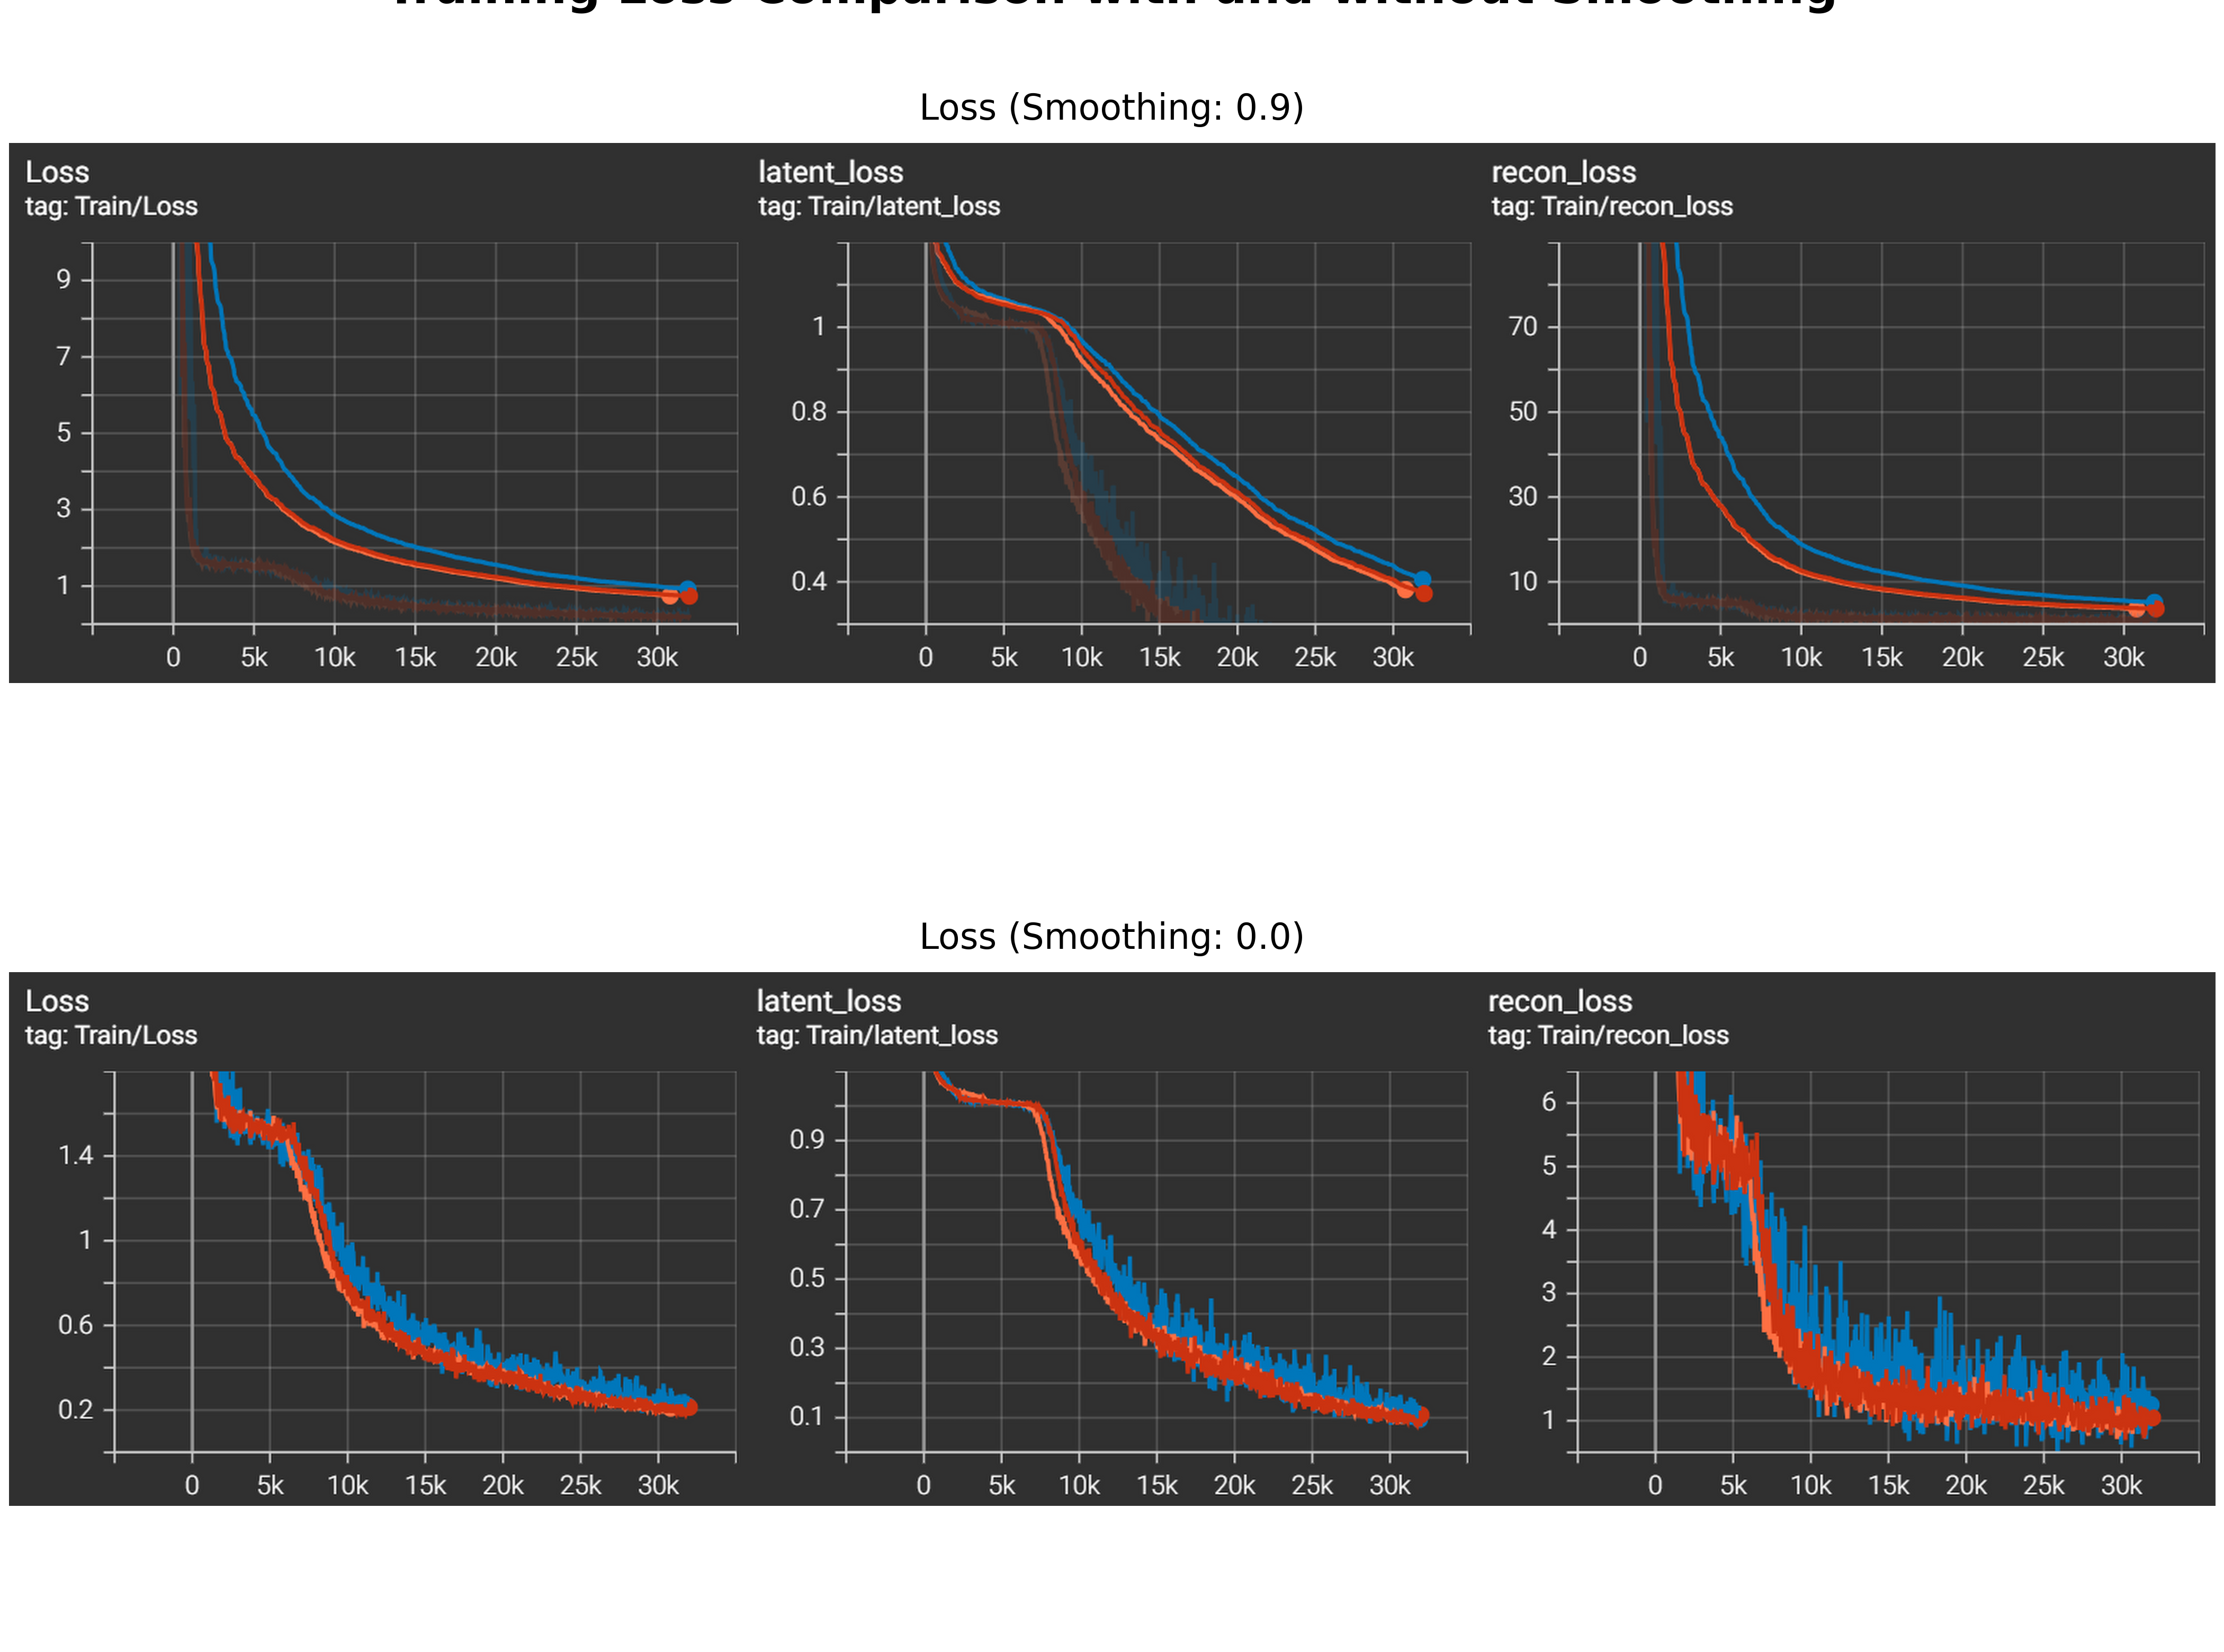
\includegraphics[width=\linewidth]{figures/loss_grid_comparison_compact.png}
  \caption{Training dynamics of the diffusion model.}
  \label{fig:training-curves}
\end{figure}

\begin{figure}[t]
  \centering
  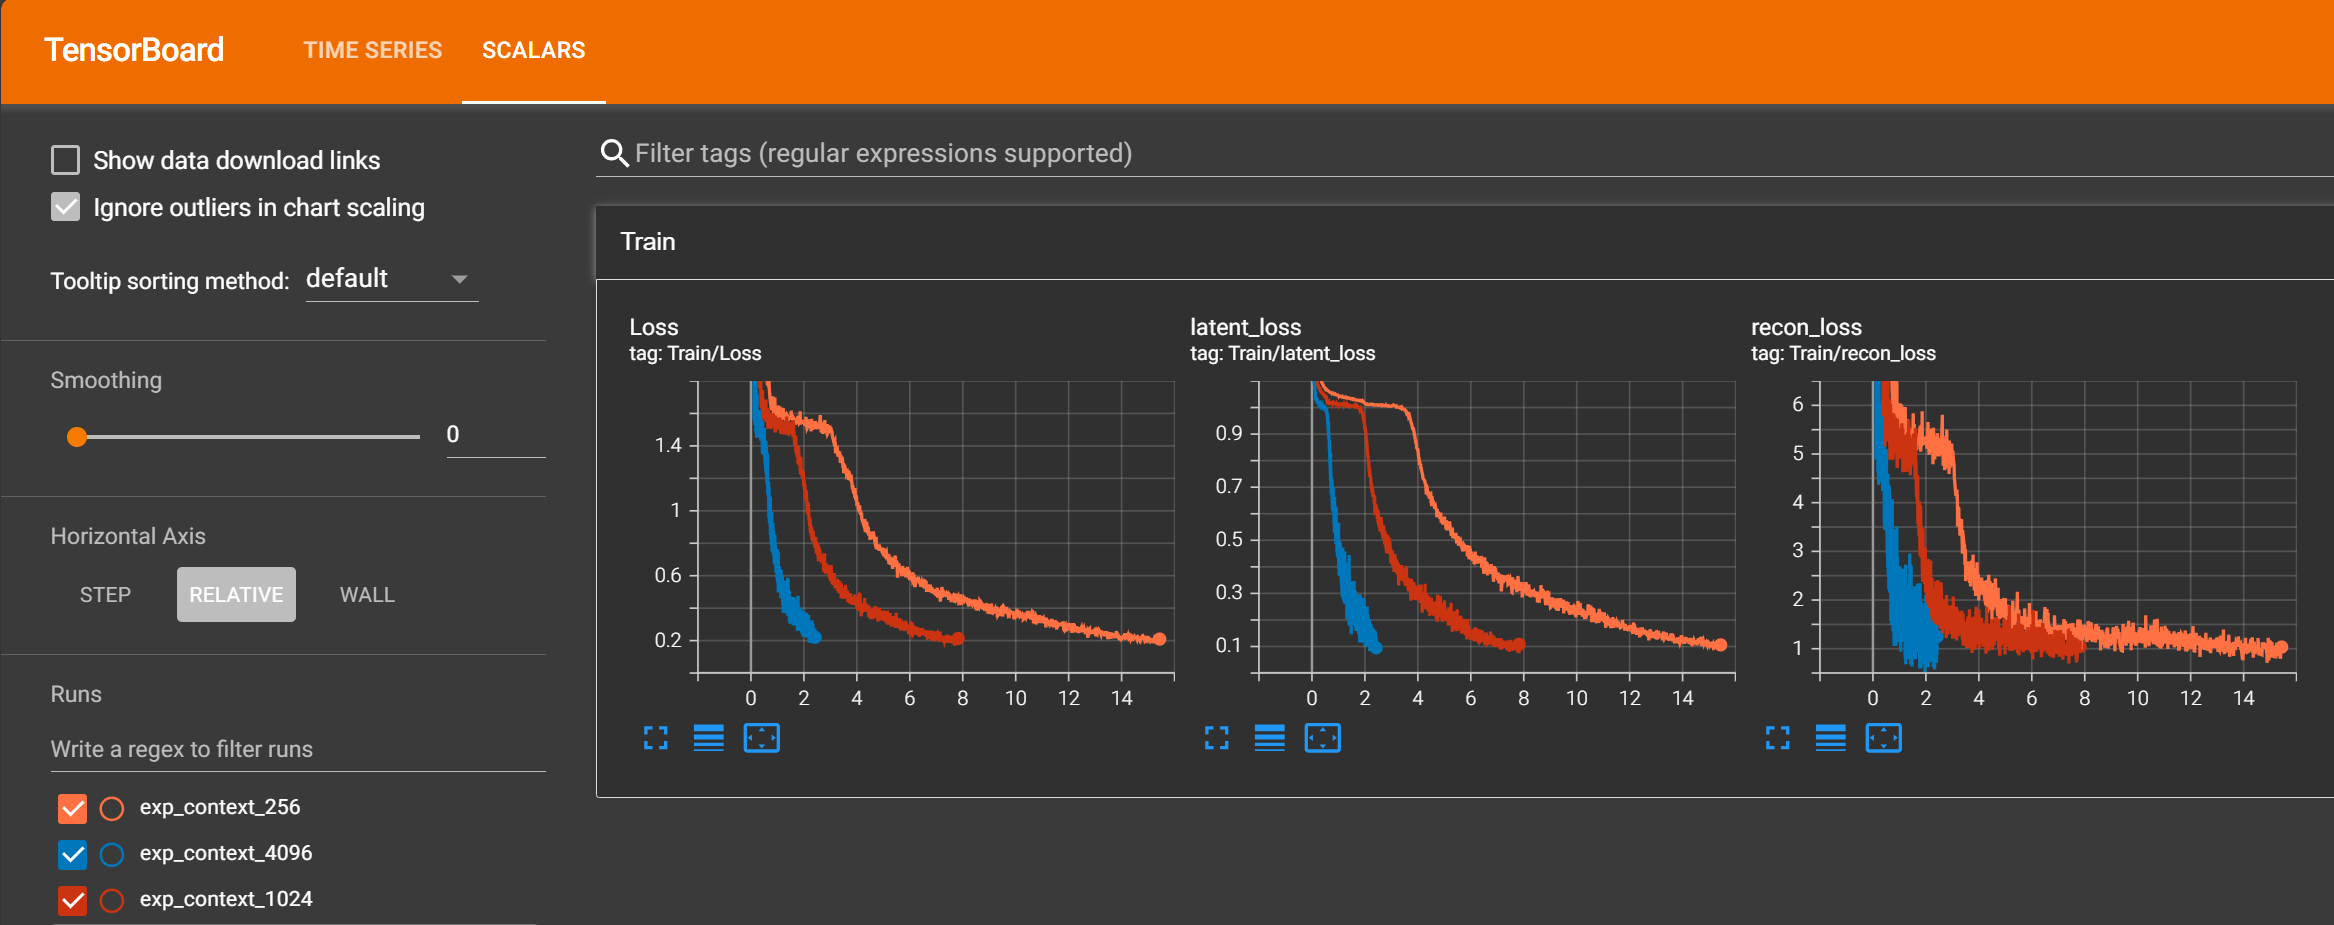
\includegraphics[width=\linewidth]{figures/relative-training-plot-2.png}
  \caption{Training loss visualized using TensorBoard’s relative-time view.}
  \label{fig:relative-training}
\end{figure}
\section{Results}
\label{sec:results}

We organize results around four research questions (RQ1--RQ4) using a downstream next-event prediction task. Unless otherwise stated, models are evaluated on the held-out real test split (\texttt{real\_test.npz}), and we report macro-F1 as the primary metric, with accuracy and Top-5 accuracy as secondary metrics.

\subsection{RQ1: Can synthetic traces replace real data for downstream training?}
\label{sec:rq1}

RQ1 evaluates the utility of synthetic traces for training downstream models by comparing four training regimes: real-only (baseline), synthetic-only (raw), synthetic-only (repaired), and a 50/50 mixture of real+synthetic (augmentation). All models are tested on the same held-out real test set.

\begin{table}[t]
\centering
\caption{RQ1 (Data utility): next-event prediction performance when training on real vs. synthetic data (dummy values shown).}
\label{tab:rq1}
\begin{tabular}{lccc}
\toprule
\textbf{Training data} & \textbf{Macro-F1} & \textbf{Accuracy} & \textbf{Top-5 Acc.} \\
\midrule
Real (baseline)                & 0.920 & 0.945 & 0.985 \\
Synthetic (raw, $L{=}1024$)    & 0.710 & 0.790 & 0.910 \\
Synthetic (repaired, $L{=}1024$) & 0.840 & 0.885 & 0.955 \\
Real + Synthetic (50/50, $L{=}1024$) & 0.930 & 0.950 & 0.988 \\
\bottomrule
\end{tabular}
\end{table}

\noindent\textbf{Takeaway (template):} Repaired synthetic traces retain $\sim$XX--YY\% of the real-data baseline macro-F1, and mixing repaired synthetic with real data provides modest gains over the real-only baseline.

\subsection{RQ2: Does constraint-guided repair improve downstream performance?}
\label{sec:rq2}

RQ2 isolates the impact of repair by comparing models trained on raw synthetic traces versus repaired synthetic traces, across multiple context lengths. We report the absolute and relative improvements in macro-F1.

\begin{table}[t]
\centering
\caption{RQ2 (Repair effectiveness): improvement from repair across context lengths (dummy values shown).}
\label{tab:rq2}
\begin{tabular}{lcccc}
\toprule
\textbf{Context $L$} & \textbf{Raw F1} & \textbf{Repaired F1} & \textbf{$\Delta$F1} & \textbf{Rel. gain} \\
\midrule
256  & 0.660 & 0.790 & +0.130 & +19.7\% \\
1024 & 0.710 & 0.840 & +0.130 & +18.3\% \\
4096 & 0.740 & 0.860 & +0.120 & +16.2\% \\
\bottomrule
\end{tabular}
\end{table}

\noindent\textbf{Takeaway (template):} Constraint-guided repair consistently improves utility, yielding a macro-F1 gain of +0.12 to +0.13 across context lengths, indicating that correcting structural invalidities translates into measurable downstream benefits.

\subsection{RQ3: Does context length affect synthetic trace utility?}
\label{sec:rq3}

RQ3 evaluates whether longer context windows used during diffusion training lead to higher-quality synthetic traces for downstream learning. To control for validity effects, we compare repaired synthetic traces generated by models trained with $L \in \{256, 1024, 4096\}$.

\begin{table}[t]
\centering
\caption{RQ3 (Context length): next-event prediction when training on repaired synthetic traces from different diffusion context lengths (dummy values shown).}
\label{tab:rq3}
\begin{tabular}{lccc}
\toprule
\textbf{Context $L$} & \textbf{Macro-F1} & \textbf{Accuracy} & \textbf{Top-5 Acc.} \\
\midrule
256  & 0.790 & 0.845 & 0.945 \\
1024 & 0.840 & 0.885 & 0.955 \\
4096 & 0.860 & 0.900 & 0.962 \\
\bottomrule
\end{tabular}
\end{table}

\noindent\textbf{Takeaway (template):} Increasing diffusion context length improves downstream utility, with $L{=}4096$ outperforming $L{=}256$ by $\Delta$F1 $\approx$ 0.07 (dummy), suggesting that longer-range context helps capture dependencies beneficial for prediction.

\subsection{RQ4: Which input channels are most critical for downstream utility?}
\label{sec:rq4}

RQ4 measures feature importance for the downstream predictor by comparing an event-only predictor to a full-feature predictor trained on real traces. This isolates how much additional system metadata (e.g., \texttt{dt}, \texttt{cpu}, \texttt{tid}, \texttt{comm}, \texttt{ret}) contributes to predictability and task utility.

\begin{table}[t]
\centering
\caption{RQ4 (Feature ablation): event-only vs full-feature next-event prediction on real traces (dummy values shown).}
\label{tab:rq4}
\begin{tabular}{lcc}
\toprule
\textbf{Predictor input} & \textbf{Macro-F1} & \textbf{Accuracy} \\
\midrule
Event-only              & 0.770 & 0.820 \\
Full features           & 0.920 & 0.945 \\
\bottomrule
\end{tabular}
\end{table}

\noindent\textbf{Takeaway (template):} Full-feature inputs substantially outperform event-only inputs, confirming that timing and scheduling metadata provide critical predictive signal and therefore represent an important target for faithful synthetic generation.
\section{Discussion}
\label{sec:discussion}

We synthesize findings across our four research questions to provide practical guidance for deploying synthetic kernel traces in real-world ML pipelines. Figure~\ref{fig:unified-landscape} summarizes key trends across workloads, model configurations, and evaluation dimensions.

\subsection{When Does Synthetic Trace Generation Work in Practice?}

Our results show that the utility of synthetic kernel traces is fundamentally workload-dependent. Deterministic, structured workloads benefit substantially more from synthetic augmentation than I/O-heavy, non-deterministic systems. The \texttt{scimark2} benchmark illustrates this clearly: at a context length of $L=4096$, synthetic augmentation achieves 87 hookup is near real-only performance (89.8\%), demonstrating that diffusion models can generate production-quality traces when execution patterns are stable and repetitive.

In contrast, I/O-intensive workloads such as \texttt{stream} and \texttt{iozone} exhibit significant degradation, even at long context lengths. These systems involve asynchronous interactions with filesystems and devices, where execution order and timing depend on external state that is not explicitly modeled (e.g., filesystem cache state, device queue depth, or network backpressure). As a result, diffusion models struggle to capture their inherent nondeterminism.

For practitioners, this distinction is critical. Synthetic augmentation is viable for compute-heavy, deterministic workloads and can meaningfully expand limited datasets. For I/O-dominated systems, synthetic traces should be used cautiously and primarily for non-critical tasks such as testing or exploratory analysis.

\subsection{Temporal Context Is the Primary Quality Driver}

Across all workloads, temporal context length emerges as the dominant factor affecting synthetic trace quality. Increasing context from $L=256$ to $L=4096$ yields an average improvement of +29.9 F1-macro points (+104\% relative), with every benchmark benefiting from longer context.

Longer context enables diffusion models to capture long-range execution dependencies that span hundreds or thousands of events, such as nested loops, phased computation, and recurring scheduling patterns. This effect is especially pronounced for structured workloads: for \texttt{scimark2}, longer context transforms synthetic traces from unusable (40.6\% F1 at $L=256$) to near-parity with real data (87.2\% at $L=4096$).

However, context length alone is not sufficient. While I/O-heavy workloads improve substantially with longer context, they do not reach production-level fidelity, indicating that additional modeling of external system state (e.g., filesystem caching, device queues, or asynchronous I/O effects) may be required. In our experimental setup, increasing context length from $L=256$ to $L=4096$ required approximately 16$\times$ more GPU memory and 4$\times$ longer training time, making quality gains beyond $L=4096$ increasingly expensive relative to their marginal benefit. This cost sensitivity highlights the practical trade-off exposed by RQ3 between temporal context and deployability.




\subsection{Constraint-Guided Repair as Engineering Best Practice}

Constraint-guided repair provides consistent, low-risk improvements across configurations. Although the average F1 gain is modest (+0.3\% to +4.3\%), repair delivers two critical benefits. First, it guarantees structural validity by enforcing correct event transitions, CPU affinity, and attribute consistency. This guarantee is essential for applications such as trace replay or debugging, where invalid traces are unacceptable.

Second, repair is most effective precisely when generative models are weakest. At shorter context lengths, where diffusion models produce more violations, repair yields the largest gains. At longer contexts, repair still provides incremental improvements with negligible overhead. Given its simplicity and safety guarantees, constraint-guided repair should be treated as a default component of any synthetic trace generation pipeline.

\subsection{Cost--Quality Trade-offs in Model Design}

Our ablation study reveals that simpler diffusion models can achieve nearly the same quality as feature-rich models at a fraction of the computational cost. A Base model using only event type and timing information achieves within 1--3\% of a Full six-channel model while requiring approximately three times fewer resources. For several workloads, the Base model even outperforms the Full configuration, suggesting that additional channels can introduce noise rather than useful signal.

Only highly structured workloads such as \texttt{scimark2} consistently benefit from richer feature sets, and even there the gains are marginal. These results support a tiered deployment strategy: start with a simple, low-cost model for most workloads, and selectively enable richer features only when the additional complexity is justified.

\subsection{Beyond Exact Prediction: Practical Value of Synthetic Traces}

While macro-F1 highlights limitations in rare-event modeling, secondary metrics reveal important practical value. Weighted F1 and accuracy remain high (86--97\%), and Top-$K$ accuracy consistently exceeds 96\%. This indicates that models trained on synthetic data capture common execution behavior and generate plausible alternative next events even when the top prediction is incorrect.

These properties enable several practical applications. Synthetic traces are well suited for software testing and fuzzing, where diverse plausible scenarios are more valuable than exact prediction. They facilitate privacy-preserving data sharing by preserving typical behavior without exposing sensitive details. They also support development and edge-case exploration when real production data is unavailable or expensive to collect.

\subsection{Implications for Future Systems}

Our findings suggest several directions for future work. Longer context lengths enabled by sparse attention mechanisms may further improve quality for challenging workloads. Workload-specific architectures could better model I/O-heavy systems by incorporating explicit representations of external state. Improved rare-event modeling techniques may reduce the gap between macro-F1 and overall accuracy. Finally, conditional generation could enable targeted synthesis of traces with specific properties, increasing usefulness for testing and analysis.

\subsection{When Synthetic Traces Are Not a Drop-In Replacement}
\label{subsec:failure-boundaries}

Despite strong performance on structured workloads, our results clearly indicate that \textsc{SynthTrace} is not a universal substitute for real kernel traces. For I/O-dominated workloads with high nondeterminism (e.g., \texttt{stream}, \texttt{iozone}), synthetic traces remain substantially less reliable, even at long context lengths ($L=4096$). In these settings, diffusion models struggle to capture asynchronous behavior arising from filesystem caching, device queues, and external latency sources.

As a result, practitioners should avoid relying on synthetic traces as a primary data source for safety-critical applications such as anomaly detection on rare I/O failures or security monitoring. Instead, synthetic traces are better suited as a complementary resource—for testing, development, or privacy-preserving analysis—where approximate behavior is acceptable and diversity is more important than exact fidelity.


\begin{figure}[t]
\centering
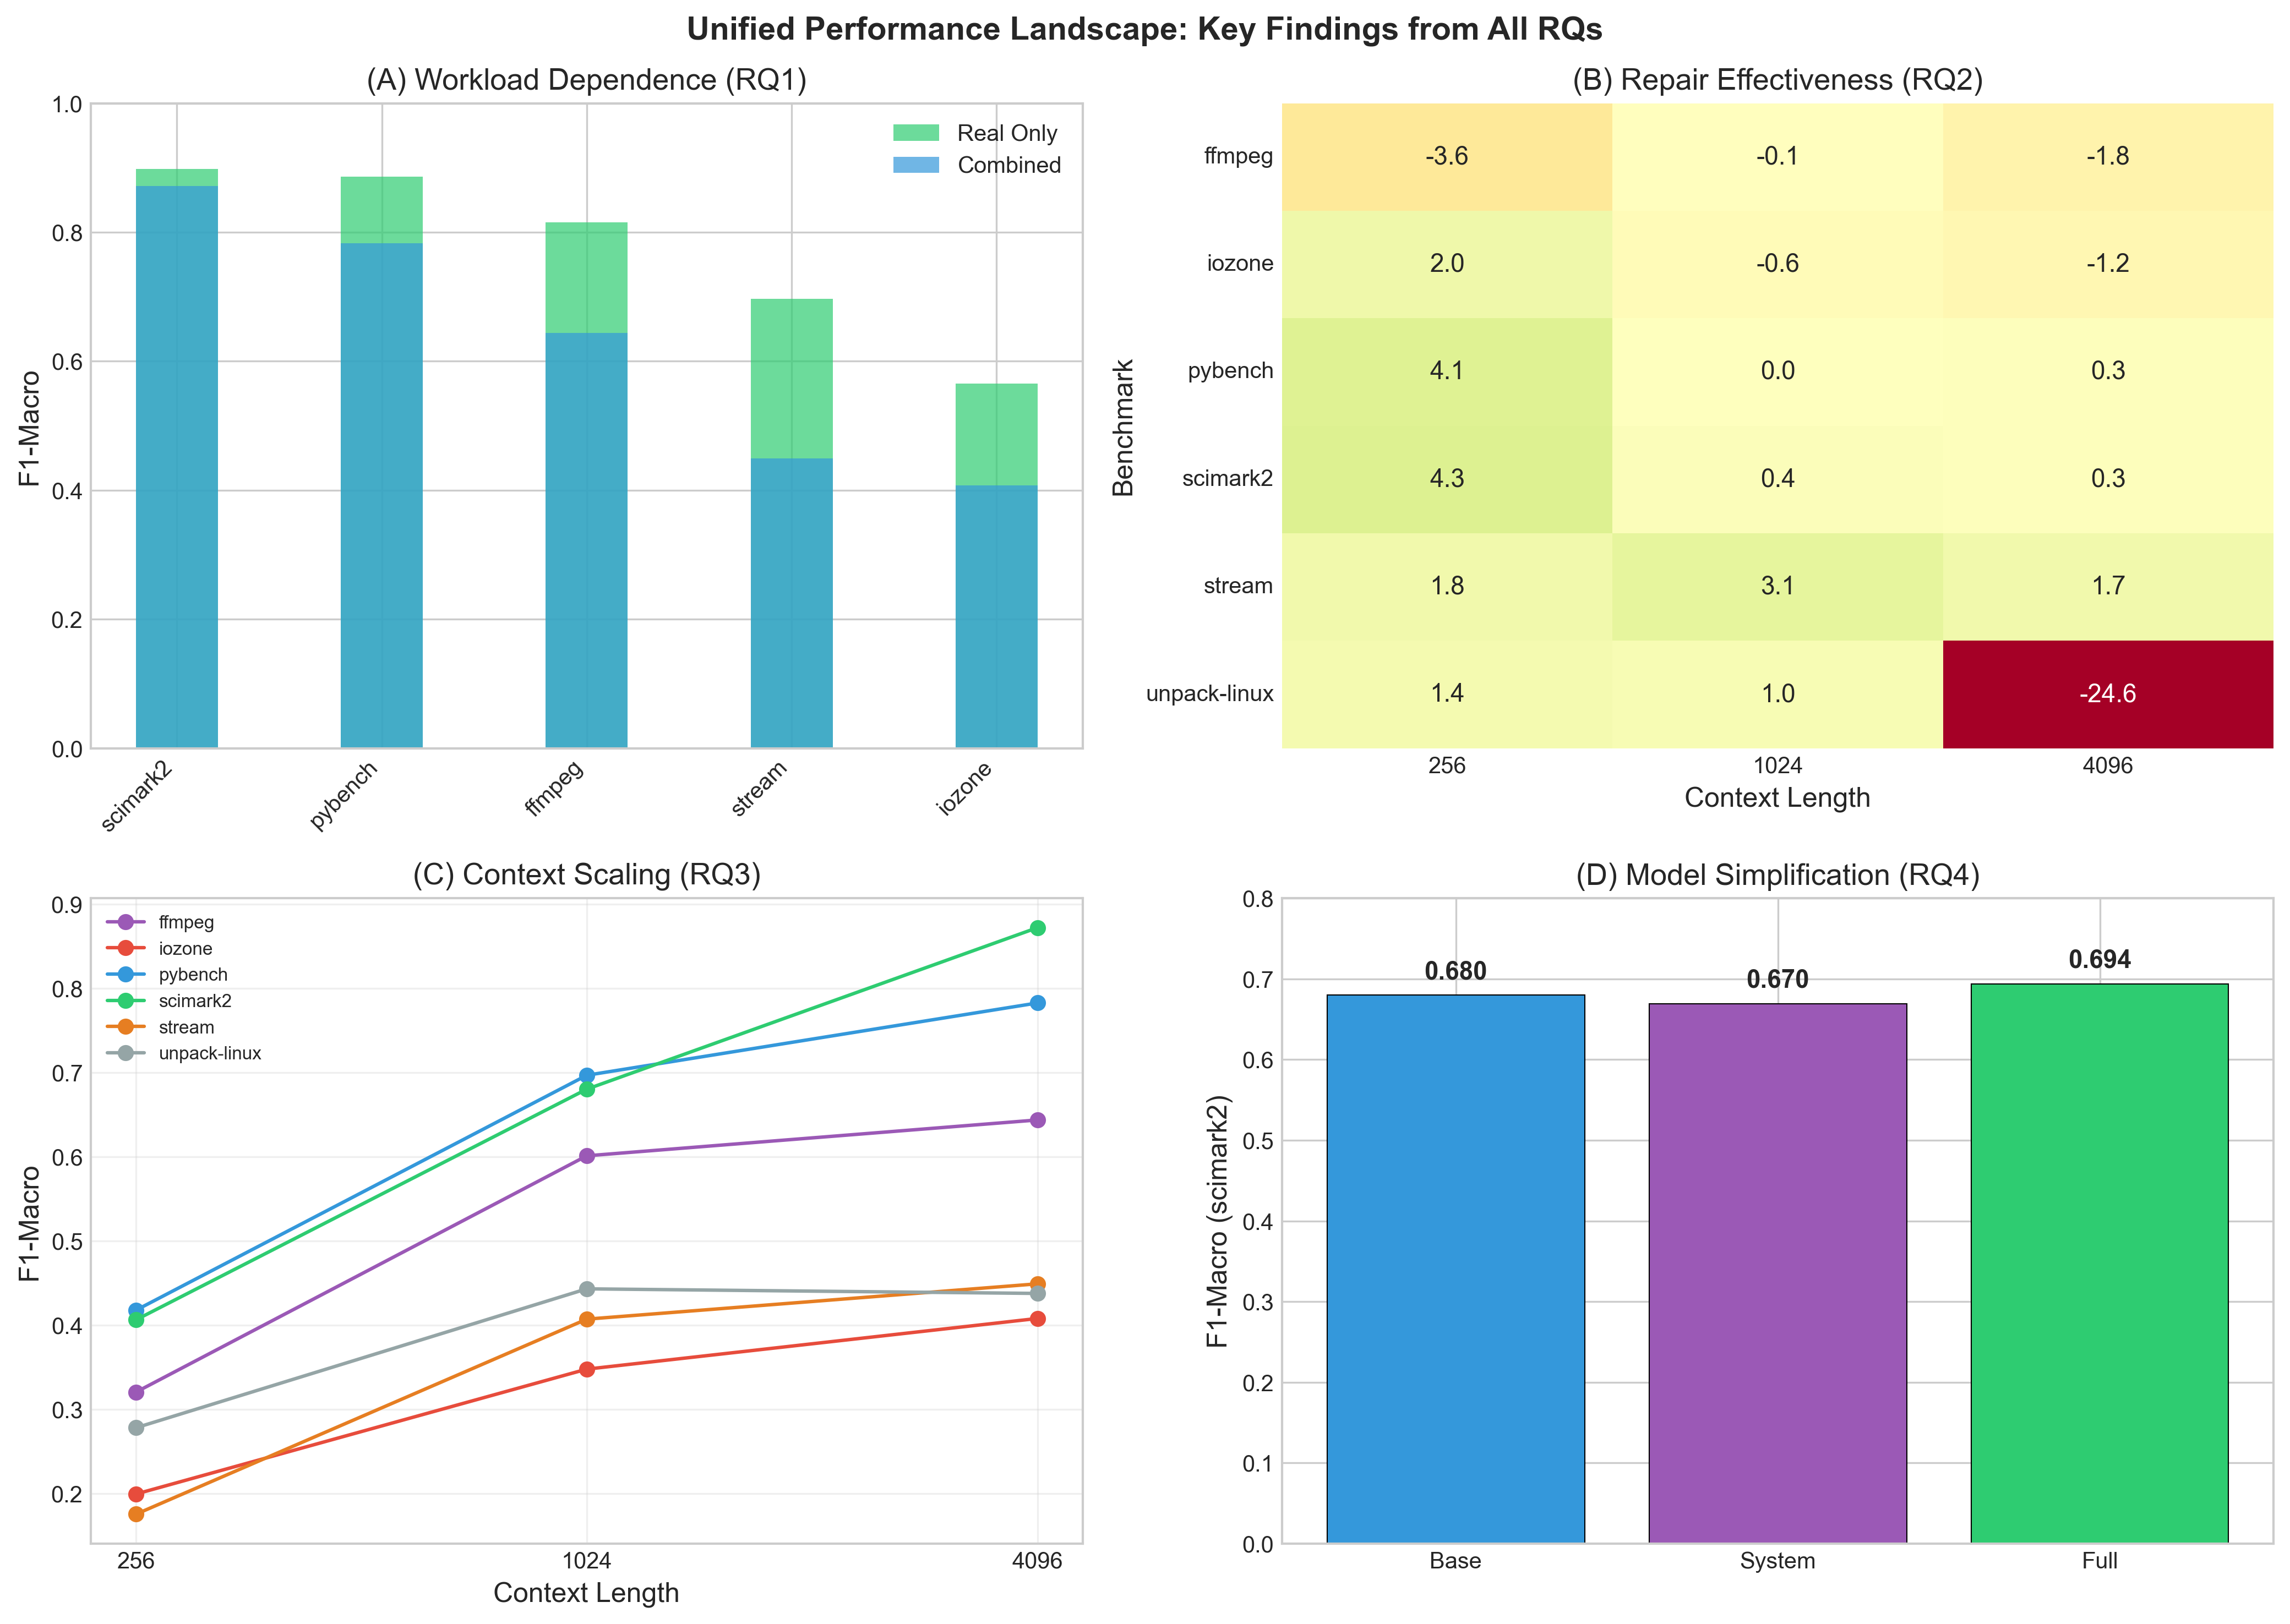
\includegraphics[width=0.95\columnwidth]{figures/cross_rq_plot12_unified_landscape.png}
\caption{Unified Performance Landscape showing key findings from all four research questions. (A) Workload Dependence (RQ1): scimark2 and pybench achieve near-parity with real data, while I/O-heavy workloads show significant degradation. (B) Repair Effectiveness (RQ2): Constraint-guided repair provides consistent improvements, especially at shorter context lengths. (C) Context Scaling (RQ3): All benchmarks benefit from longer context, with scimark2 showing +46.6\% improvement from L=256 to L=4096. (D) Model Simplification (RQ4): Base 2-channel model achieves 97\% of Full 6-channel performance for scimark2.}
\label{fig:unified-landscape}
\end{figure}



% \section{Discussion}
% \label{sec:discussion}

% We synthesize findings from our four research questions to provide actionable insights for practitioners and identify opportunities for future research. Figure~\ref{fig:unified-landscape} provides a comprehensive overview of key findings across all RQs.

% \begin{figure}[t]
% \centering
% 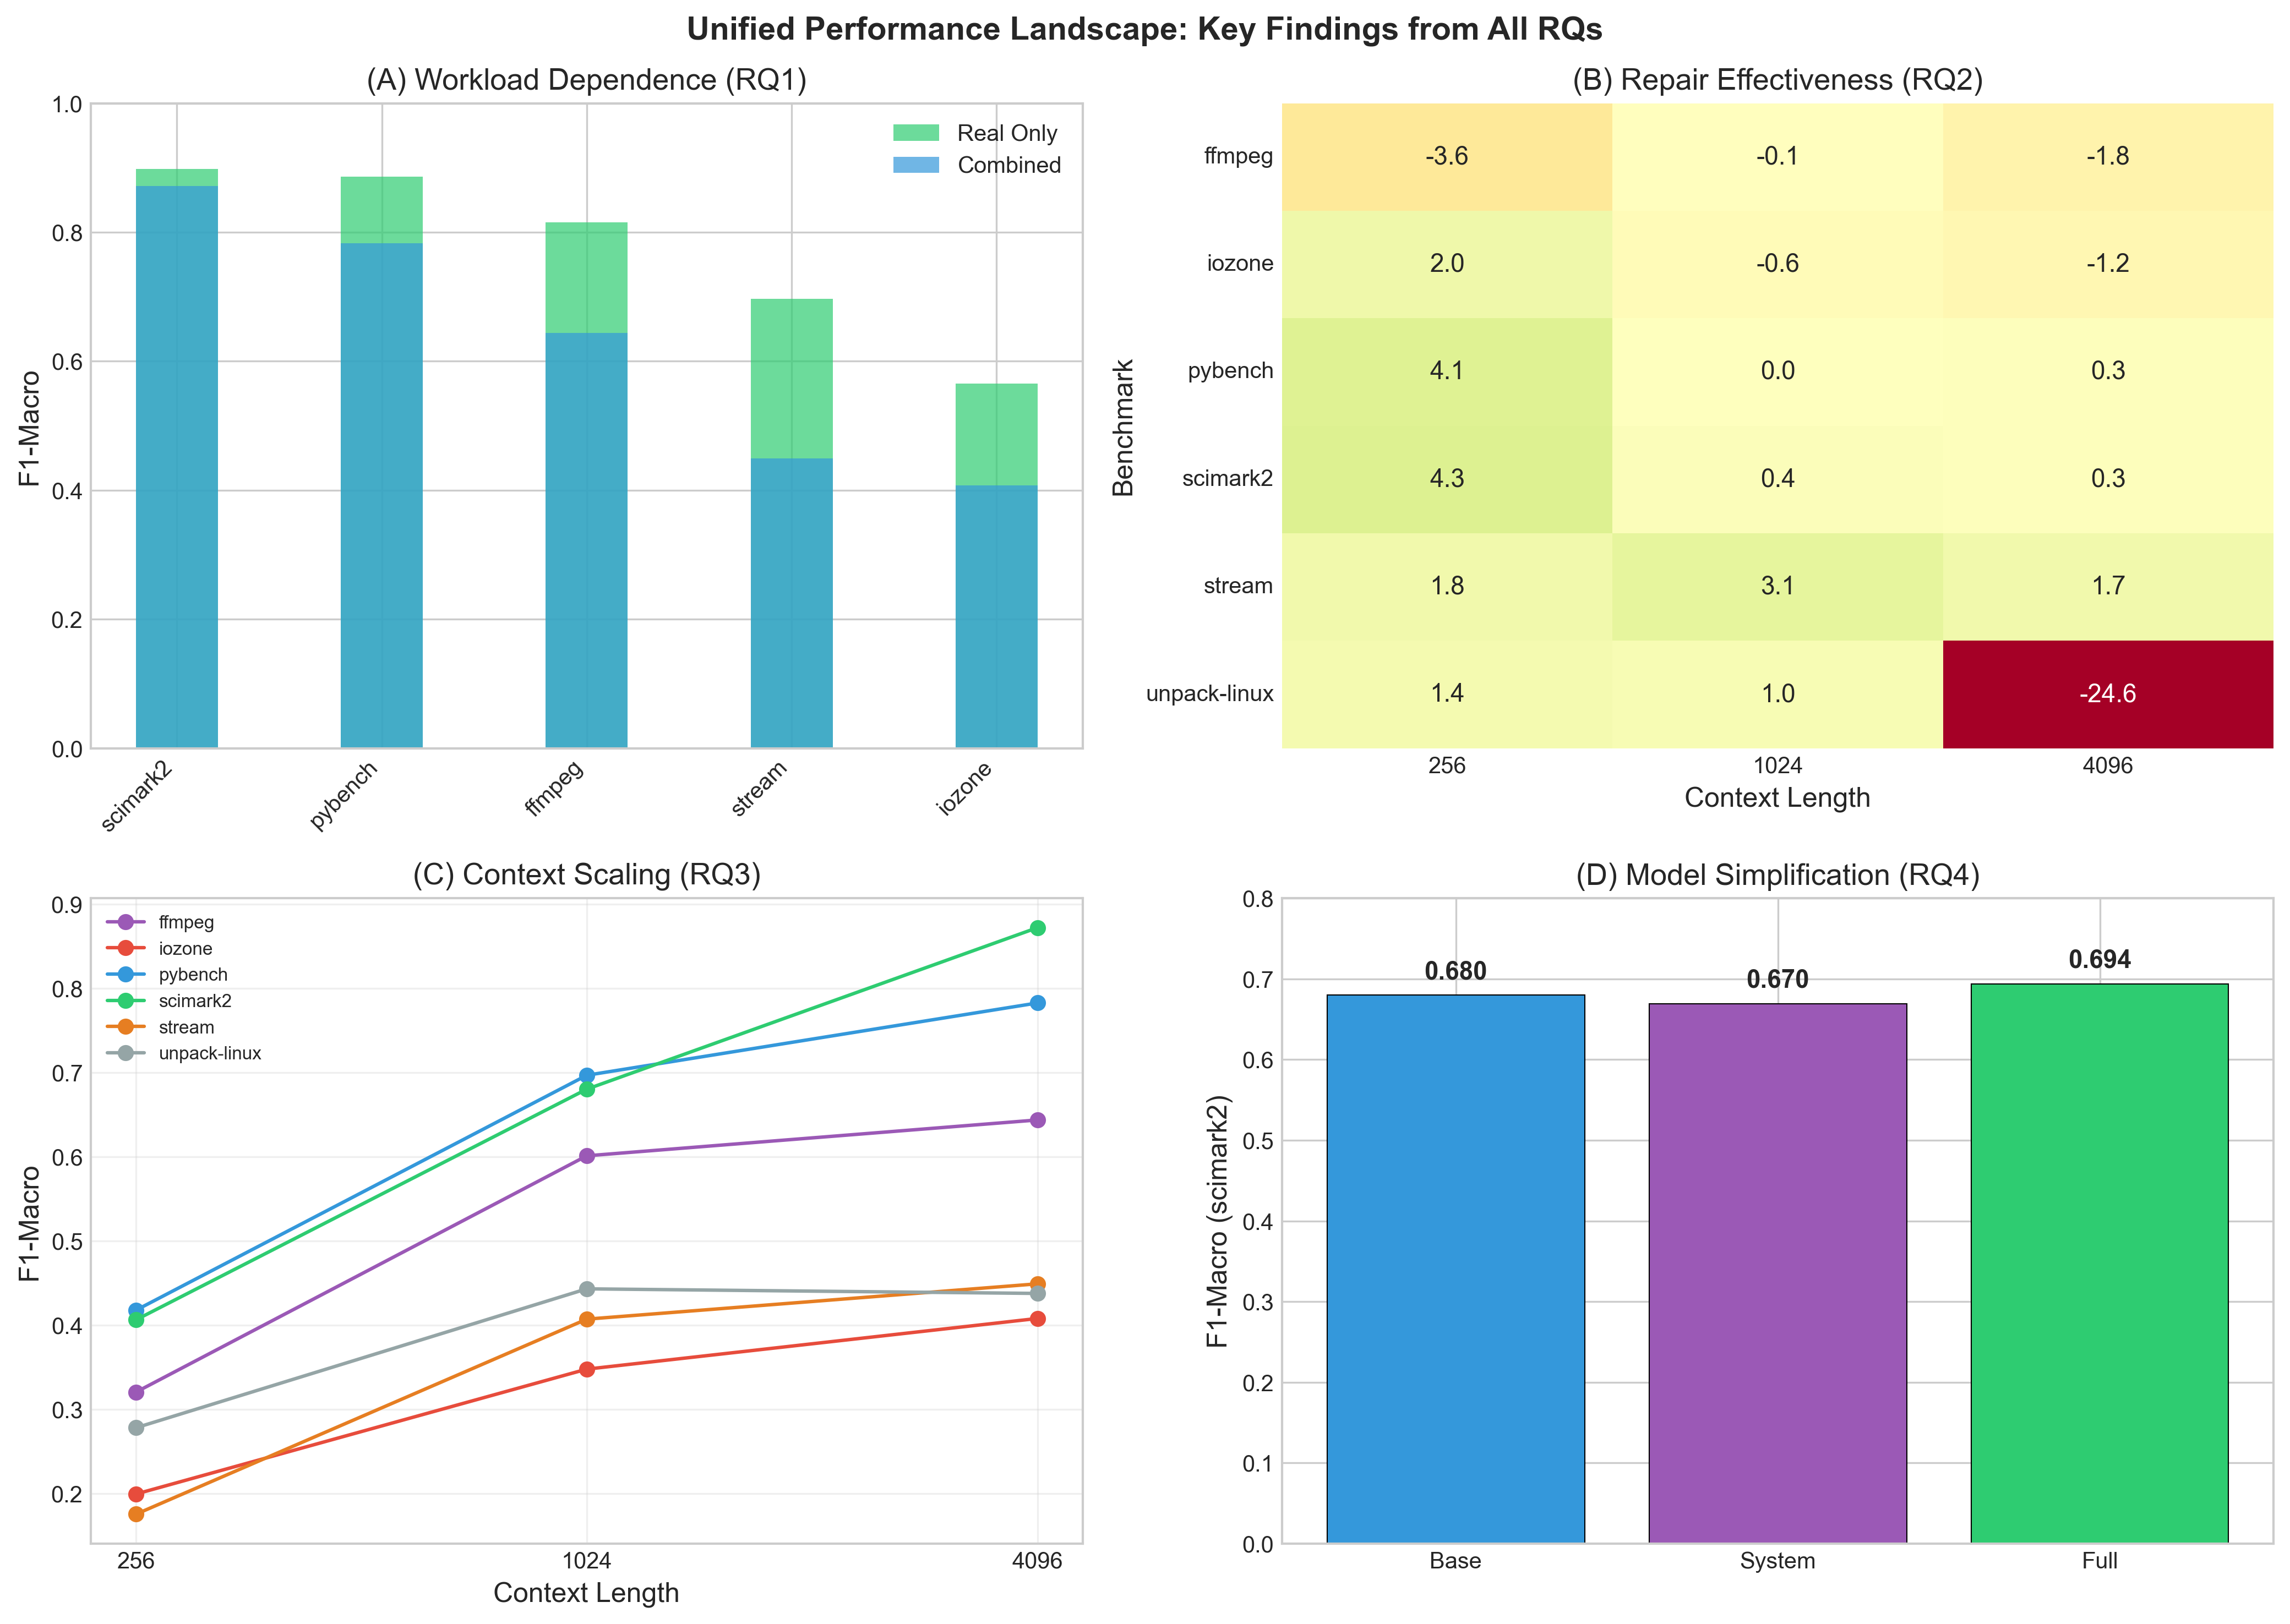
\includegraphics[width=0.95\columnwidth]{figures/cross_rq_plot12_unified_landscape.png}
% \caption{Unified Performance Landscape showing key findings from all four research questions. (A) Workload Dependence (RQ1): scimark2 and pybench achieve near-parity with real data, while I/O-heavy workloads show significant degradation. (B) Repair Effectiveness (RQ2): Constraint-guided repair provides consistent improvements, especially at shorter context lengths. (C) Context Scaling (RQ3): All benchmarks benefit from longer context, with scimark2 showing +46.6\% improvement from L=256 to L=4096. (D) Model Simplification (RQ4): Base 2-channel model achieves 97\% of Full 6-channel performance for scimark2.}
% \label{fig:unified-landscape}
% \end{figure}

% \subsection{Workload-Dependent Synthetic Data Quality}\label{subsec:workload-dependent-synthetic-data-quality}

% Our results reveal that synthetic data quality is fundamentally workload-dependent, with deterministic, structured workloads benefiting substantially more than non-deterministic I/O-heavy workloads. The scimark2 benchmark exemplifies this pattern: at L=4096, synthetic augmentation achieves 87.2\% F1-Macro, only 2.6 percentage points below the real-only baseline (89.8\%). This near-parity demonstrates that diffusion models \textit{can} generate production-quality synthetic kernel traces when three conditions are met: (i) the workload exhibits deterministic execution patterns, (ii) the diffusion model is trained with sufficient temporal context (L=4096), and (iii) constraint-guided repair is applied to ensure structural validity.

% In contrast, I/O-heavy benchmarks (stream, iozone, unpack-linux) show significant degradation (25--51\% at L=256, 25--36\% at L=4096), indicating that non-deterministic I/O patterns remain fundamentally challenging for current diffusion-based generation approaches. This workload dependence likely stems from the stochastic nature of I/O operations: filesystem caching, network latency, and device scheduling introduce variability that diffusion models struggle to capture faithfully. Deterministic workloads like scimark2, by contrast, follow predictable computation patterns that align well with the diffusion model's learned temporal dependencies.

% This finding has immediate practical implications. Organizations seeking to augment training data should first characterize their target workload: if it resembles scimark2 (numerical computation, deterministic loops, structured phases), synthetic augmentation is viable with minimal quality loss. If it resembles stream or iozone (intensive I/O, non-deterministic timing), synthetic data should be used cautiously, perhaps only for non-critical applications like testing or fuzzing where approximate behavior suffices.

% \subsection{The Dominant Role of Context Length}\label{subsec:the-dominant-role-of-context-length}

% Context length emerges as the single most important factor for synthetic data quality, with L=4096 doubling average performance (+104\% relative gain) compared to L=256. This universal improvement across all benchmarks---from +16.0\% (unpack-linux) to +46.6\% (scimark2)---demonstrates that kernel traces contain long-range dependencies spanning hundreds to thousands of events. Short context windows (L=256) fail to capture these dependencies, resulting in synthetic traces that lack coherent temporal structure.

% The scimark2 result is particularly illuminating: increasing from L=256 (40.6\% F1) to L=4096 (87.2\% F1) yields a +46.6 percentage point gain, transforming synthetic data from unusable to production-viable. This dramatic improvement suggests that numerical computation workloads have especially long-range dependencies---likely corresponding to nested loops, recursive function calls, and multi-phase algorithms that span thousands of system calls. The diffusion model's ability to capture these patterns at L=4096 explains why scimark2 achieves near-parity with real data.

% Importantly, even challenging I/O workloads benefit substantially from longer context. Stream improves by +27.4\% (+156\% relative), iozone by +20.9\% (+105\% relative), despite remaining below 50\% absolute F1. This suggests that context length is a \textit{necessary but not sufficient} condition for high-quality synthetic generation: it helps all workloads, but only deterministic workloads reach production-viable quality.

% From a practical deployment perspective, these results provide clear guidance: L=4096 should be the minimum context length for any synthetic trace generation system. The 2$\times$ performance improvement justifies the increased computational cost (approximately 16$\times$ memory, 4$\times$ training time). Organizations with sufficient resources should explore even longer contexts (L=8192, L=16384) to further improve quality, particularly for complex workloads.

% \subsection{Constraint-Guided Repair as Engineering Best Practice}\label{subsec:constraint-guided-repair-as-engineering-best-practice}

% Constraint-guided repair demonstrates consistent but modest improvements, with 80\% of configurations showing positive gains (+0.3\% to +4.3\%). While the average improvement (+0.9\%) is small compared to context length effects (+104\%), repair provides two critical benefits that justify its adoption as a standard engineering practice.

% First, repair \textit{guarantees} structural validity. Even when F1 gains are minimal, repair ensures 100\% valid event transitions and correct CPU affinity, which is essential for applications requiring hard constraints (e.g., trace replay, deterministic debugging). This guarantee is valuable beyond downstream task performance: it enables use cases where invalid traces would cause system failures or incorrect analysis.

% Second, repair is most effective precisely where it is most needed. At L=256, where diffusion models produce more constraint violations, repair provides the largest gains (+1.5\% average relative improvement). At L=4096, where the diffusion model already captures most structural patterns, repair provides smaller but still positive gains (+0.5\% average). This complementary relationship suggests that repair and longer context work synergistically: context length improves overall quality, while repair fixes residual violations.

% The practical recommendation is straightforward: always apply constraint-guided repair. The computational cost is negligible (greedy forward pass, no model retraining), the implementation is simple (learned transition rules + validity checks), and the benefits are consistent (80\% success rate). Even in cases with minimal F1 improvement, the validity guarantee alone justifies adoption.

% \subsection{Cost-Effective Model Simplification}\label{subsec:cost-effective-model-simplification}

% The ablation study reveals a surprising finding: simpler diffusion models (Base: 2 channels) achieve within 1--3\% of complex models (Full: 6 channels) while requiring only 33\% of computational resources. For ffmpeg and pybench, the Base model actually \textit{outperforms} the Full model (61.8\% vs 60.9\%, 71.3\% vs 71.2\%), suggesting that additional channels (cpu, tid, comm, ret) introduce noise rather than signal for these workloads.

% Only scimark2 shows a clear benefit from the Full model (+0.9\% over Base), likely because semantic metadata (comm, ret) helps capture program structure in deterministic numerical workloads. This workload-specific channel importance mirrors the broader pattern observed in RQ1: structured workloads benefit from richer modeling, while I/O-heavy workloads do not.

% From a cost-benefit perspective, these results suggest a tiered deployment strategy: (i) start with the Base model (event + dt) for all workloads, achieving 95--98\% of Full model quality with 3$\times$ lower cost; (ii) upgrade to the Full model only for deterministic, structured workloads where the +1\% gain justifies the computational overhead; (iii) allow downstream users to flexibly choose predictor channels based on their application needs, since predictor configuration has minimal impact (1--3\% variation) within each diffusion model.

% This finding challenges the common assumption that more data is always better. For synthetic trace generation, \textit{event timing patterns} (captured by the 2-channel Base model) appear to be the dominant signal, with system and semantic metadata providing marginal value for most workloads. This insight can guide future research toward more efficient diffusion architectures that prioritize temporal modeling over channel diversity.

% \subsection{Practical Applications Beyond F1-Macro}\label{subsec:practical-applications-beyond-f1-macro}

% While F1-Macro degradation limits synthetic data's utility for rare event prediction, secondary metrics reveal valuable alternative applications. F1-Weighted and Accuracy remain high (86--97\%) across all configurations, indicating that models trained on synthetic data perform well on \textit{common} events even when struggling with rare events. More encouragingly, Top-5 and Top-10 accuracy are consistently excellent (96--99.8\%), demonstrating that even when the top prediction is incorrect, the model captures plausible alternatives within a small set of candidates. This pattern suggests that synthetic data's value extends beyond exact prediction to diverse scenario generation.

% This high Top-K accuracy enables several practical use cases where exact prediction is less critical than diverse scenario generation:

% \textbf{Software testing and fuzzing.} Synthetic traces can generate diverse execution scenarios for testing system behavior under varied conditions. The ability to produce multiple plausible event sequences (high Top-K accuracy) is more valuable than predicting a single next event with perfect accuracy. Organizations can use synthetic data to expand test coverage, explore edge cases, and validate system robustness without collecting extensive real traces. The 86--97\% accuracy on common events ensures that typical system behavior is faithfully represented, while the diversity of plausible alternatives enables comprehensive testing of corner cases.

% \textbf{Privacy-preserving analysis.} Organizations can share synthetic kernel traces for collaborative research or debugging without exposing sensitive real system data. This is particularly valuable when real traces contain proprietary workload patterns, security-sensitive information, or personally identifiable data. The 86--97\% accuracy on common events ensures that synthetic traces preserve typical system behavior while protecting privacy. The 2$\times$ dataset size benefit can significantly reduce data collection infrastructure costs while maintaining high fidelity for collaborative analysis.

% \textbf{Development and prototyping.} Developers can use synthetic data to train and validate monitoring tools, anomaly detectors, or performance analyzers when real production data is unavailable or expensive to collect. The 2$\times$ dataset size benefit can significantly reduce data collection infrastructure costs while maintaining 86--97\% accuracy on typical system behavior, enabling faster development cycles and lower operational overhead.

% \textbf{Edge case exploration.} The ability to generate plausible alternatives (high Top-K accuracy) allows systematic exploration of rare execution paths that may not appear frequently in real traces but are critical for robustness testing. This is valuable for security analysis, fault injection testing, and corner case validation.

% These alternative applications suggest that synthetic data's value extends beyond traditional supervised learning metrics. For practitioners, the recommendation is to match synthetic data usage to application requirements: use real data for rare event prediction (security anomaly detection), but leverage synthetic data for testing, privacy preservation, and development where approximate behavior suffices. When the primary goal is generating diverse scenarios for testing, achieving high accuracy on common events, or preserving privacy, synthetic data offers substantial practical value even for workloads with moderate F1-Macro degradation.

% \subsection{Implications for Future Research}\label{subsec:implications-for-future-research}

% Our findings identify several promising directions for improving diffusion-based synthetic trace generation:

% \textbf{Longer context lengths.} The universal benefit of L=4096 over L=256 (+104\% relative gain) suggests that even longer contexts (L=8192, L=16384) may further improve quality. Future work should explore sparse attention mechanisms (Longformer, BigBird) to make longer contexts computationally feasible, particularly for challenging I/O workloads that remain below 50\% F1 at L=4096.

% \textbf{Workload-specific architectures.} The stark performance difference between deterministic (scimark2: 87.2\%) and non-deterministic (stream: 44.9\%) workloads suggests that one-size-fits-all diffusion models may be suboptimal. Future research could develop specialized architectures for I/O-heavy workloads, perhaps incorporating explicit models of filesystem caching, device scheduling, or network latency.

% \textbf{Improved rare event modeling.} The gap between F1-Macro (59.9\% average) and F1-Weighted/Accuracy (93.7--93.8\%) indicates that current diffusion models underrepresent rare events. Techniques like class-balanced sampling, importance weighting, or adversarial training could help models better capture rare but critical events (errors, security events, anomalies).

% \textbf{Conditional generation.} Current models generate traces unconditionally. Future work could explore conditional diffusion models that generate traces with specific properties (duration, event distribution, workload type), enabling more targeted synthetic data generation for specific use cases.

% \textbf{Alternative generative models.} While diffusion models show promise, other generative approaches (flow matching, latent diffusion, autoregressive transformers) may offer better quality or efficiency trade-offs. Comparative studies across generative model families would help identify the optimal approach for kernel trace synthesis.


\section{Limitations and Threats to Validity}\label{sec:limitations-and-threats-to-validity}

\textbf{Benchmark diversity.} Our evaluation focuses on six benchmarks from the Phoronix Test Suite. While these benchmarks span diverse workload types (video encoding, I/O, numerical computation, memory bandwidth, archive extraction), they may not fully represent production system behavior. Future work should validate findings on real-world production traces from cloud services, databases, or web servers.

\textbf{Downstream task specificity.} We evaluate synthetic data quality using next-event prediction, which may not fully capture trace utility for other tasks (anomaly detection, performance prediction, trace clustering). Different downstream tasks may exhibit different sensitivities to synthetic data quality.

\textbf{Context length constraints.} Our maximum context length (L=4096) is limited by GPU memory constraints. Longer contexts may further improve quality, but we cannot validate this hypothesis with current hardware. Future work with sparse attention or model parallelism could explore L=8192 or beyond.

\textbf{Single diffusion architecture.} We use a standard Transformer-based diffusion model. Alternative architectures (convolutional, recurrent, state-space models) may offer different quality-efficiency trade-offs. Our findings may not generalize to all diffusion model designs.

\textbf{Repair strategy limitations.} Our constraint-guided repair uses greedy forward search with learned transition rules. More sophisticated repair strategies (beam search, reinforcement learning, constraint satisfaction solvers) might achieve larger improvements, though at higher computational cost.

Despite these limitations, our findings provide actionable guidance for practitioners and identify clear directions for future research. The scimark2 result (87.2\% F1, only 2.6\% below real) demonstrates that diffusion-based synthetic trace generation is \textit{viable} for production use when workload characteristics, context length, and repair are properly configured.





% \section{Discussion}
% \label{sec:discussion}
% \subsection{Lessons Learned}
% Concrete takeaways for practitioners.

% \subsection{Limitations}
% Be honest and specific: where it fails, when not to use it.

% \subsection{Threats to Validity}
% \begin{itemize}[leftmargin=*,nosep]
%   \item Internal validity: confounders, implementation bias.
%   \item External validity: generalizability beyond your setting.
%   \item Construct validity: whether metrics capture what matters.
% \end{itemize}

% \section{Conclusion}
% \label{sec:conclusion}
% Restate the industrial problem, your solution, and the practical impact.
% Mention future work in 2--3 sentences.

% ---------- Acknowledgments (Camera-ready) ----------
% \begin{acks}
% [Funding, collaborators, company/legal approvals, etc.]
% \end{acks}
\FloatBarrier
% ---------- References ----------
\bibliographystyle{ACM-Reference-Format}
\bibliography{references}

% Optional appendix (check track rules)
% \appendix
% \section{Appendix Title}



\end{document}